\chapter{效率评定补充图}
\label{app:efficiency-plots}

本附录收录第5章效率修正中提及的全部单对象效率映射和事例级效率图，作为正文中堆叠汇总图的补充。所有效率图均基于 DPS1 全模拟 MC 样本产生，分箱方案与正文一致。

\section{单对象接受度与条件效率}

\begin{figure}[htbp]
  \centering
  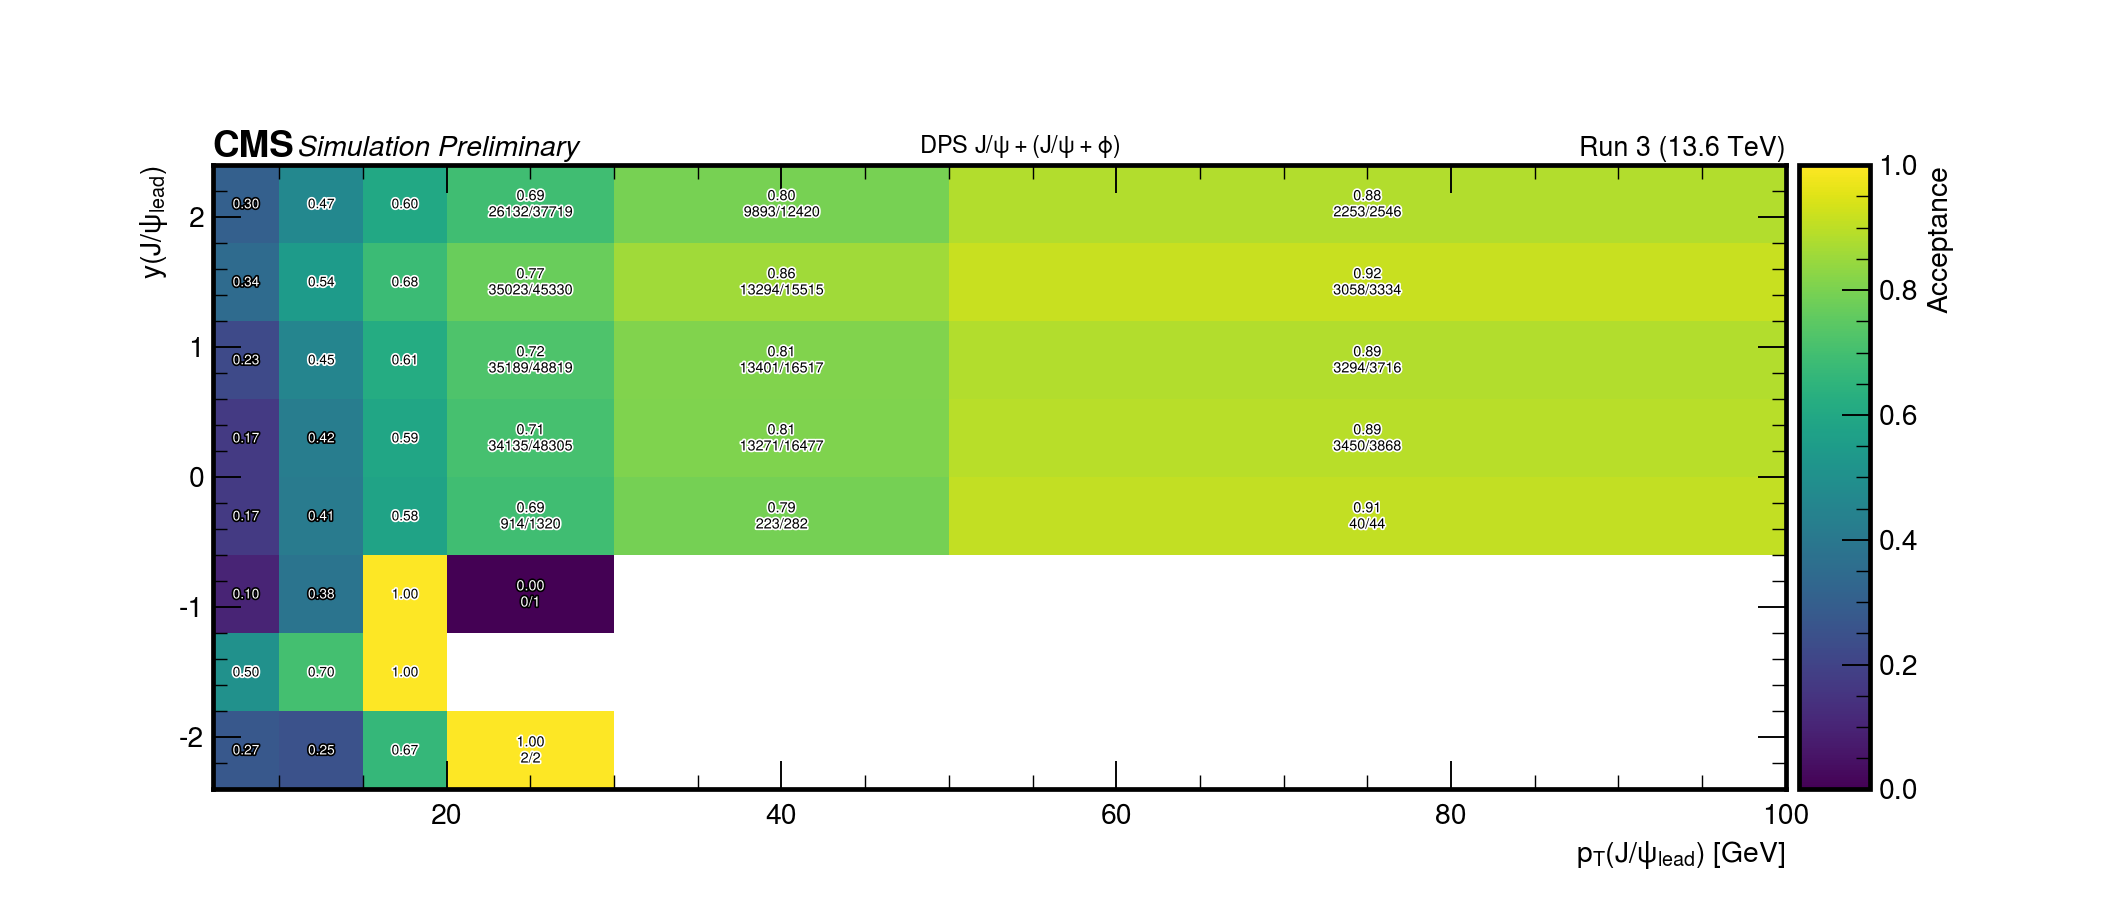
\includegraphics[width=0.85\textwidth]{figures/appendix-efficiency/object2d_jpsi_lead_fiducial_acceptance.png}\\[2pt]
  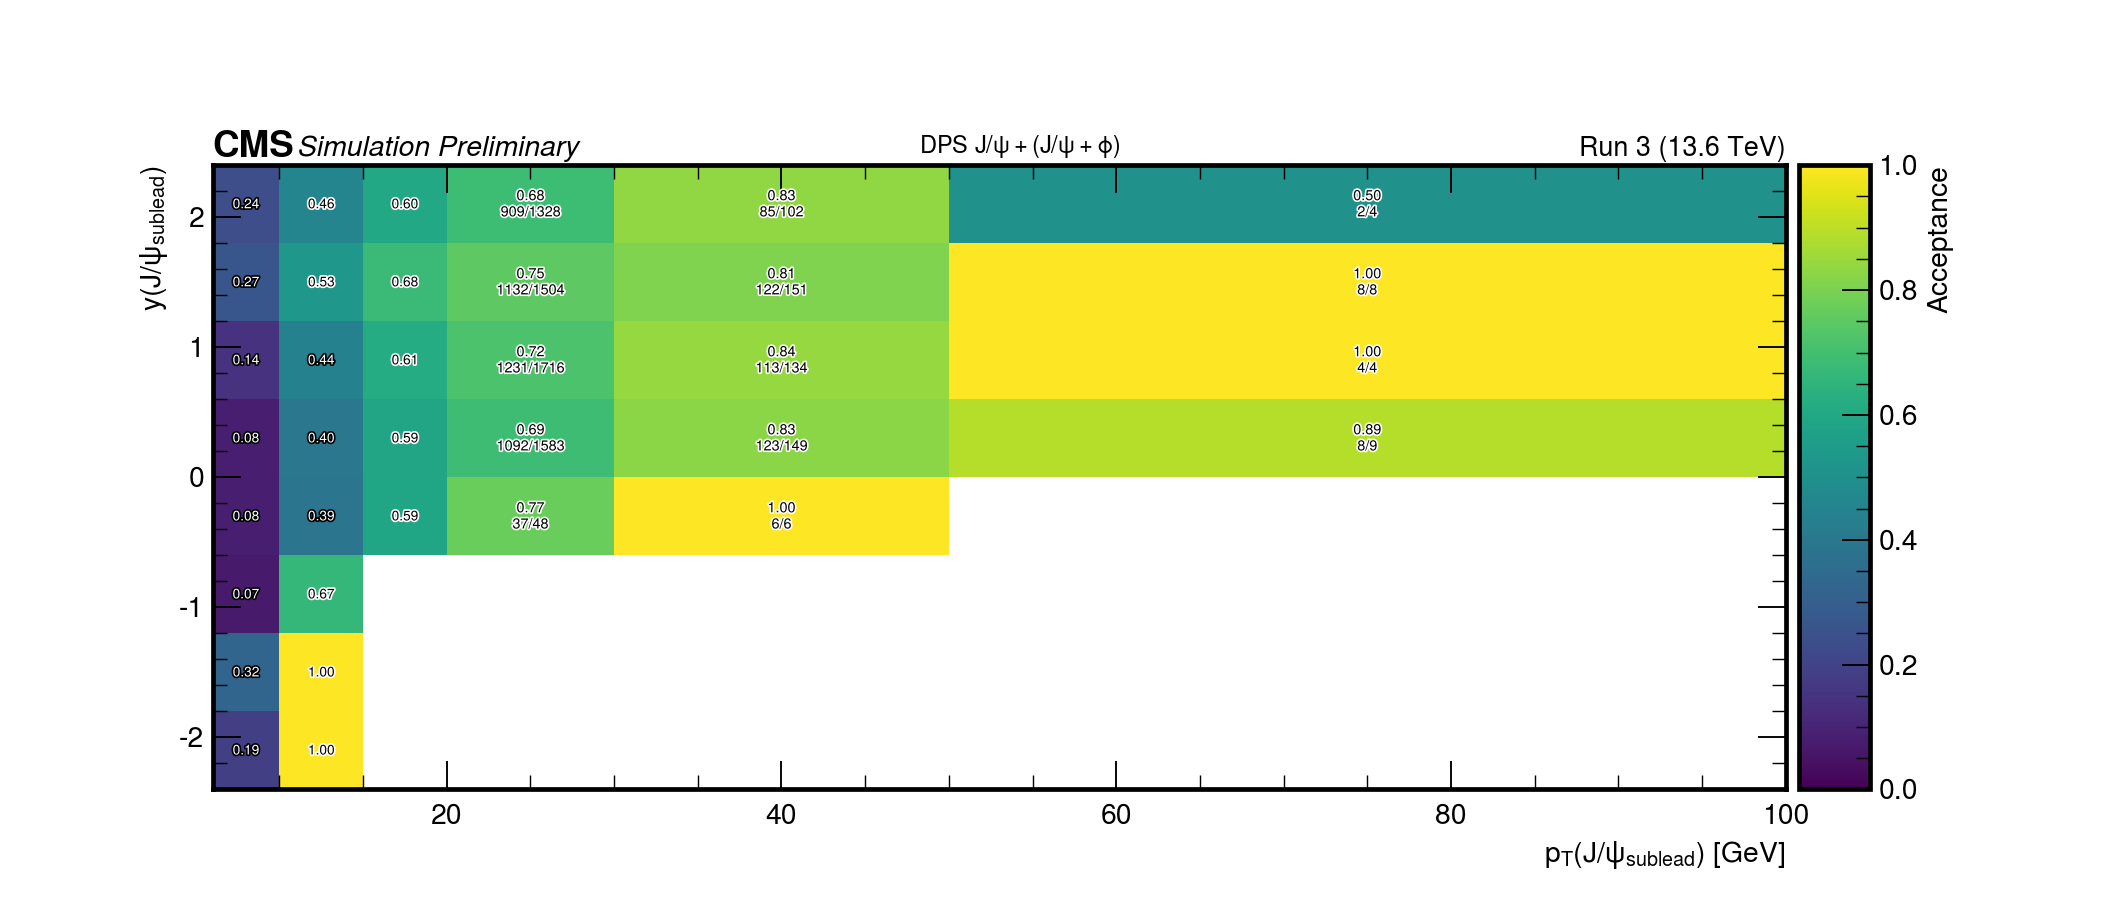
\includegraphics[width=0.85\textwidth]{figures/appendix-efficiency/object2d_jpsi_sublead_fiducial_acceptance.png}\\[2pt]
  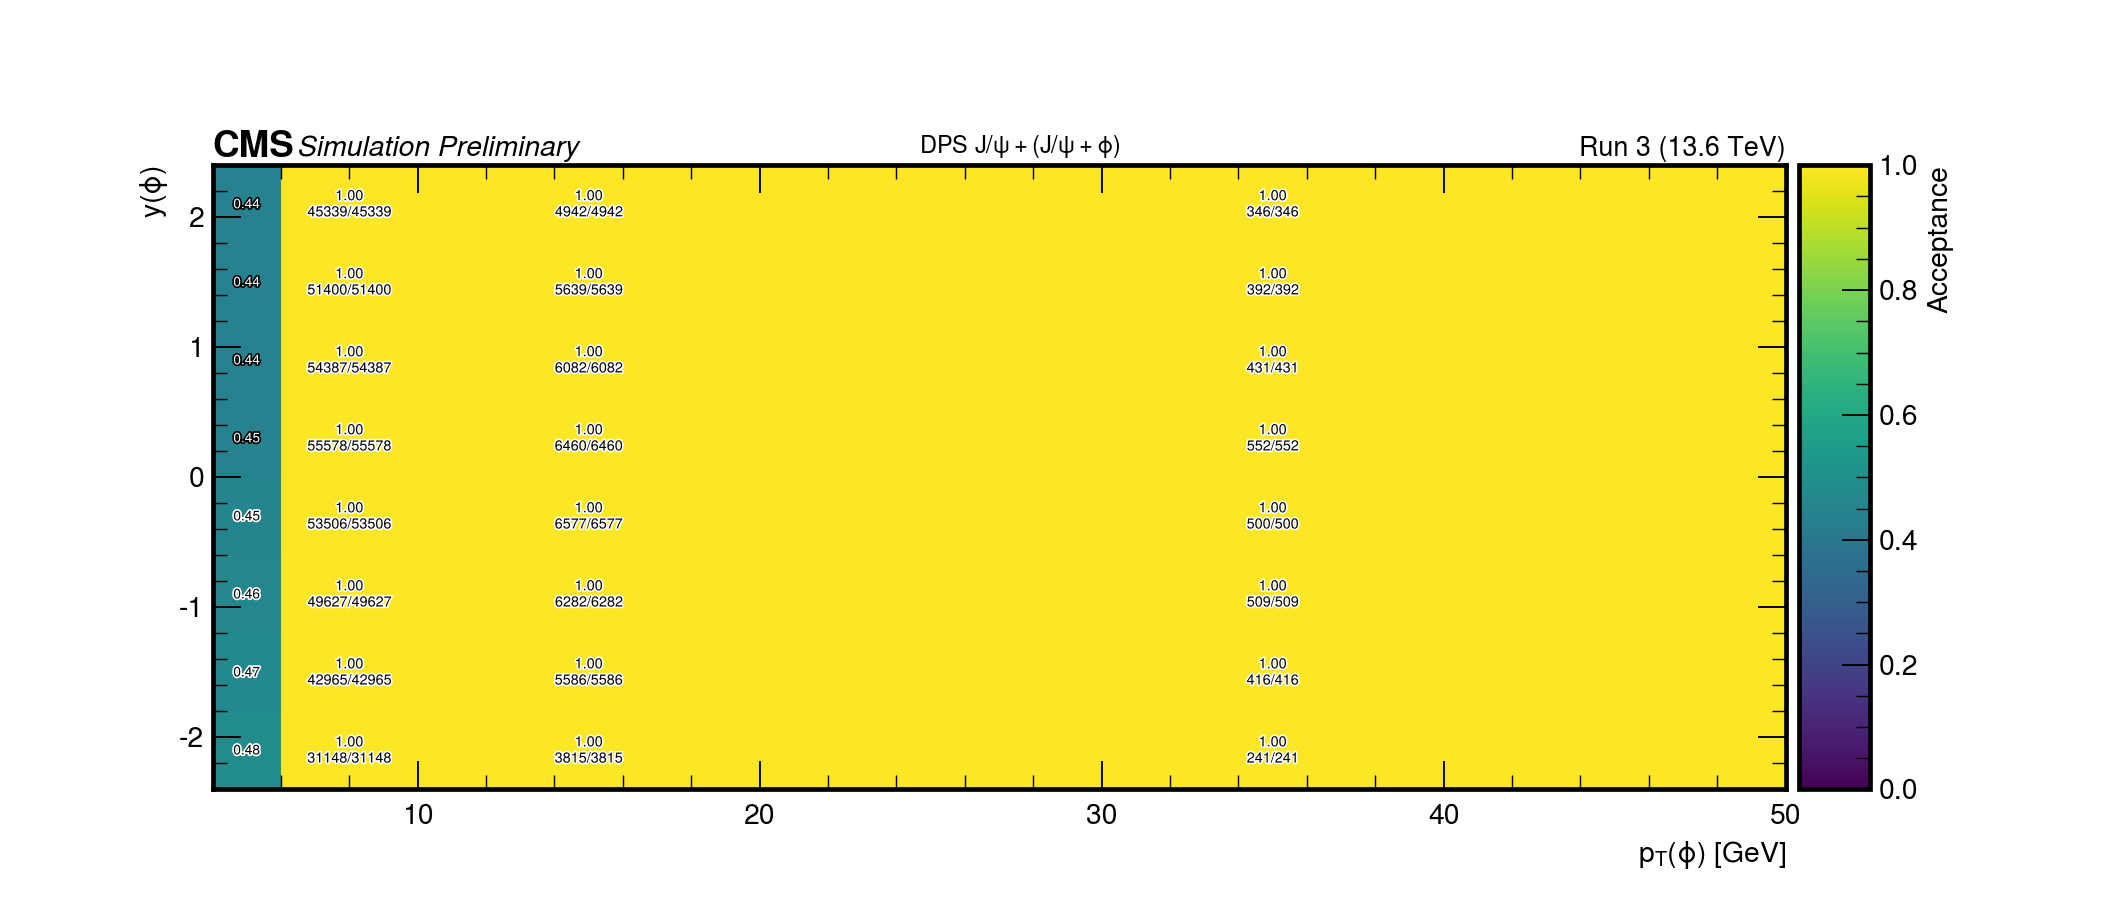
\includegraphics[width=0.85\textwidth]{figures/appendix-efficiency/object2d_phi_fiducial_acceptance.png}
  \caption{单对象基准接受度（从上至下：leading $J/\psi$、subleading $J/\psi$、$\phi$），作为各对象$(p_{\mathrm{T}}, |y|)$的函数。}
  \label{fig:app-all-obj-acceptance}
\end{figure}

\begin{figure}[htbp]
  \centering
  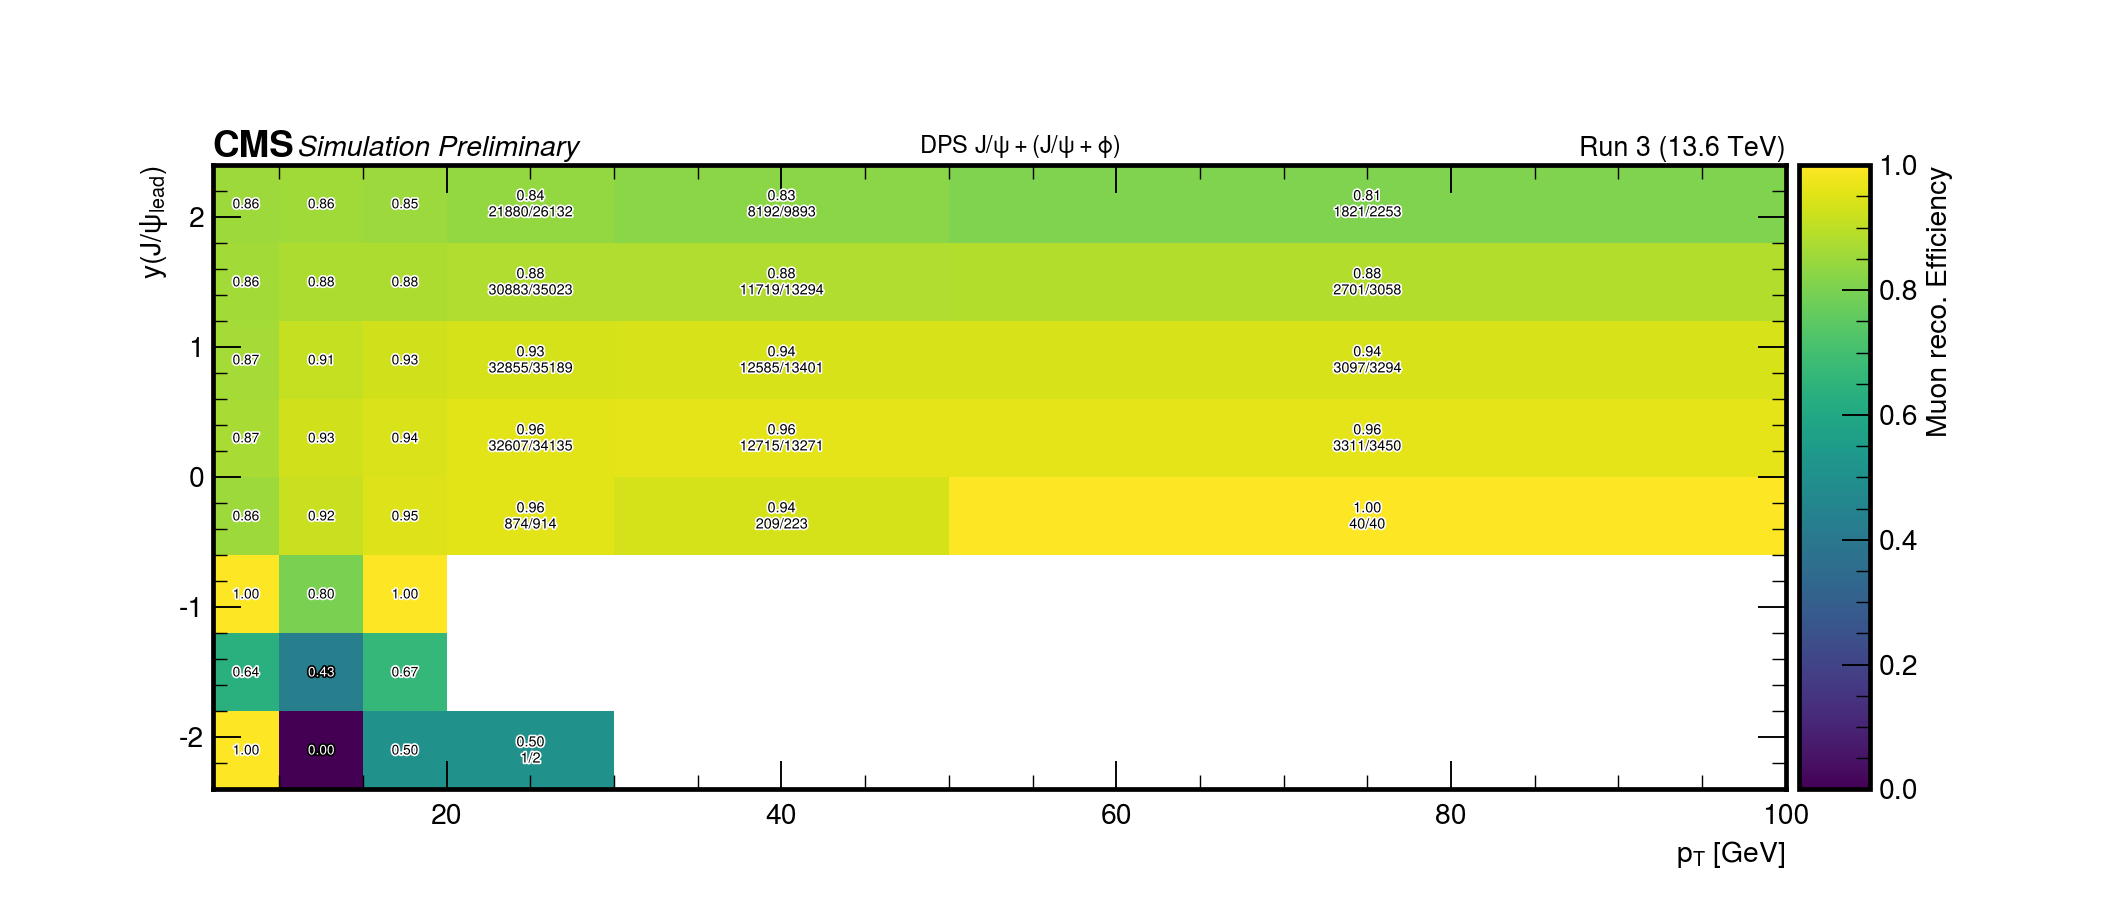
\includegraphics[width=0.85\textwidth]{figures/appendix-efficiency/object2d_jpsi_lead_muonRECO.png}\\[2pt]
  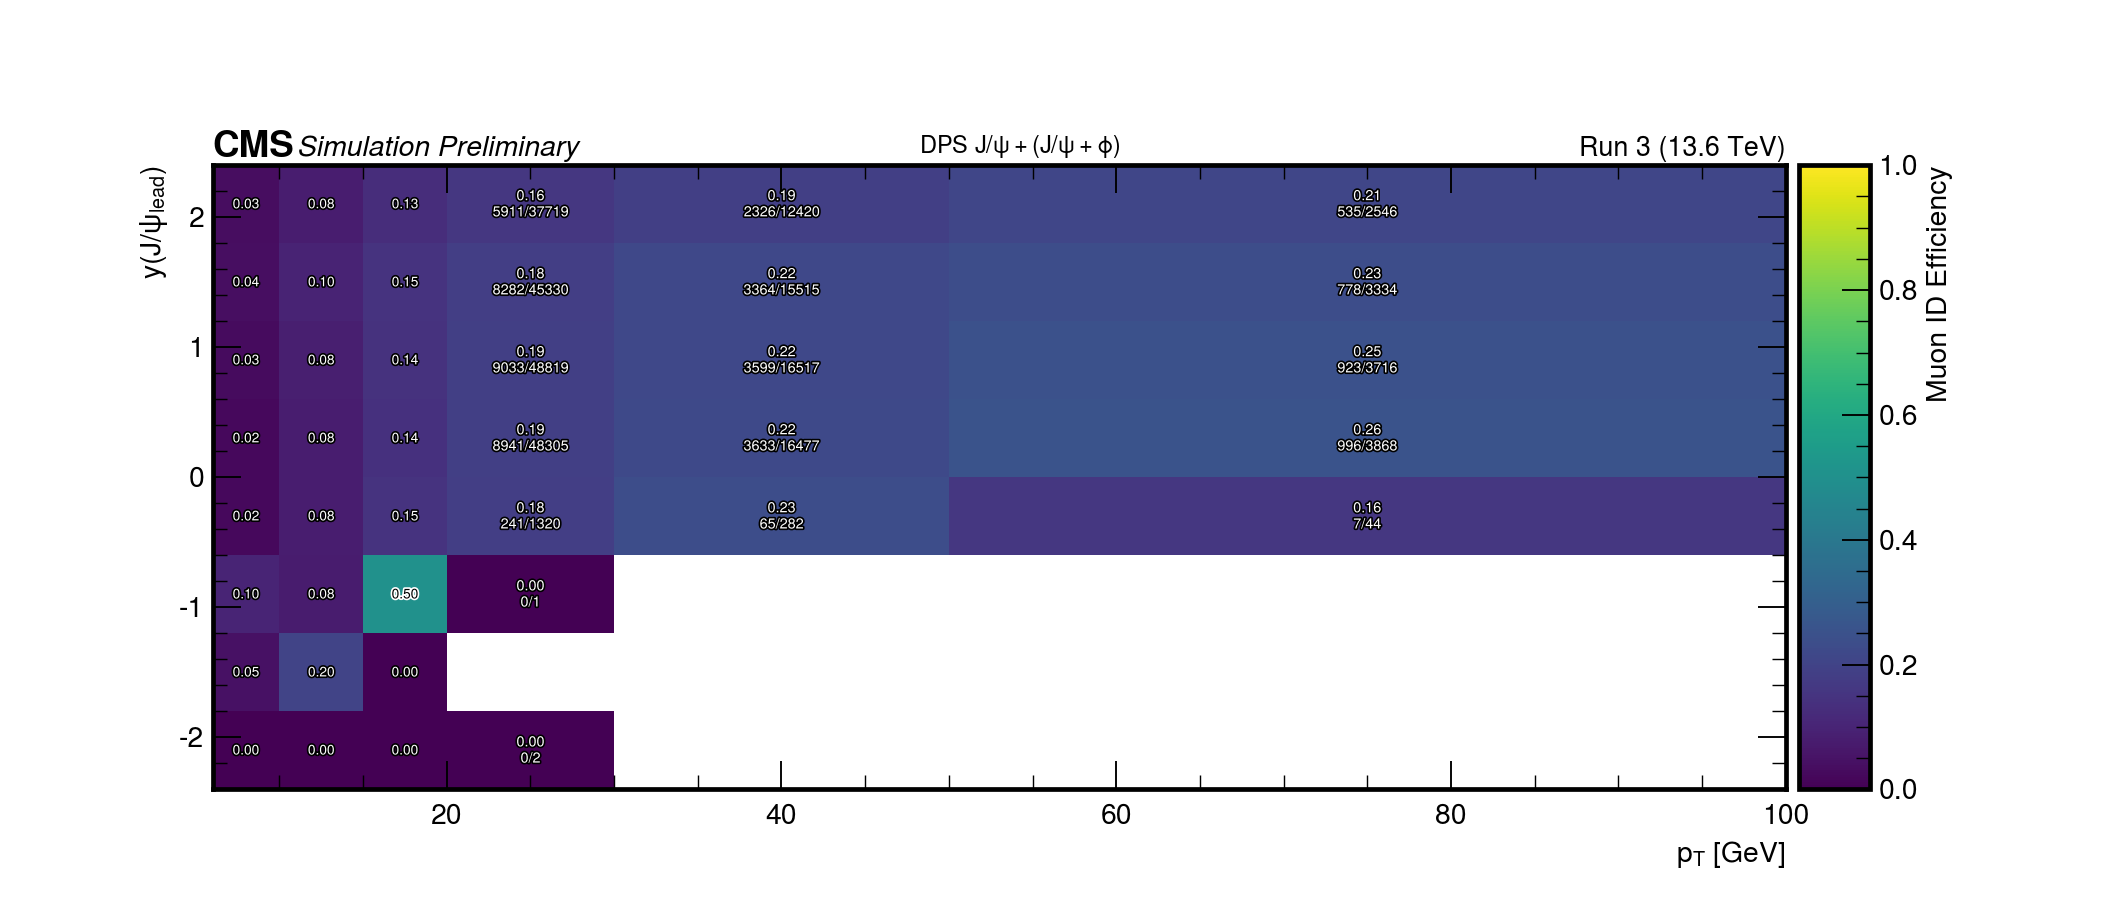
\includegraphics[width=0.85\textwidth]{figures/appendix-efficiency/object2d_jpsi_lead_muonID.png}\\[2pt]
  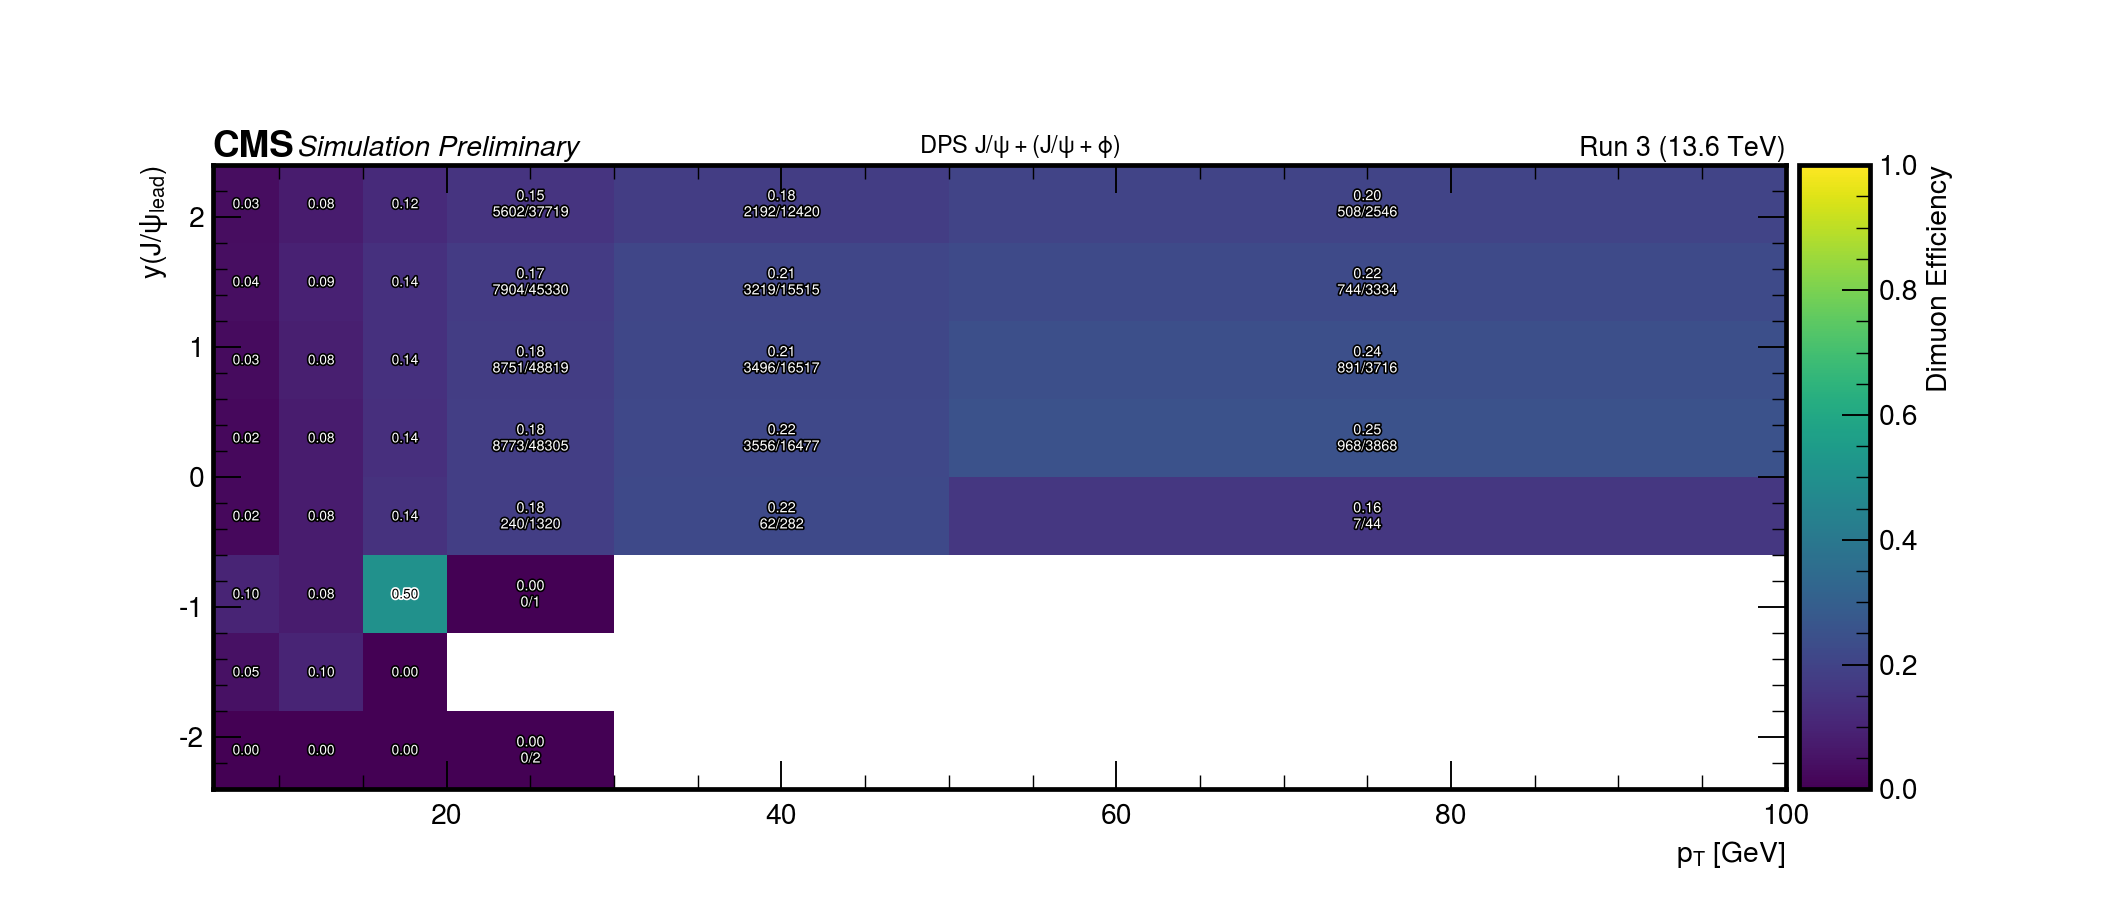
\includegraphics[width=0.85\textwidth]{figures/appendix-efficiency/object2d_jpsi_lead_dimuon.png}
  \caption{Leading $J/\psi$的条件效率（从上至下：缪子重建、缪子鉴别、双缪子选择）。}
  \label{fig:app-eff-jpsi-lead}
\end{figure}

\begin{figure}[htbp]
  \centering
  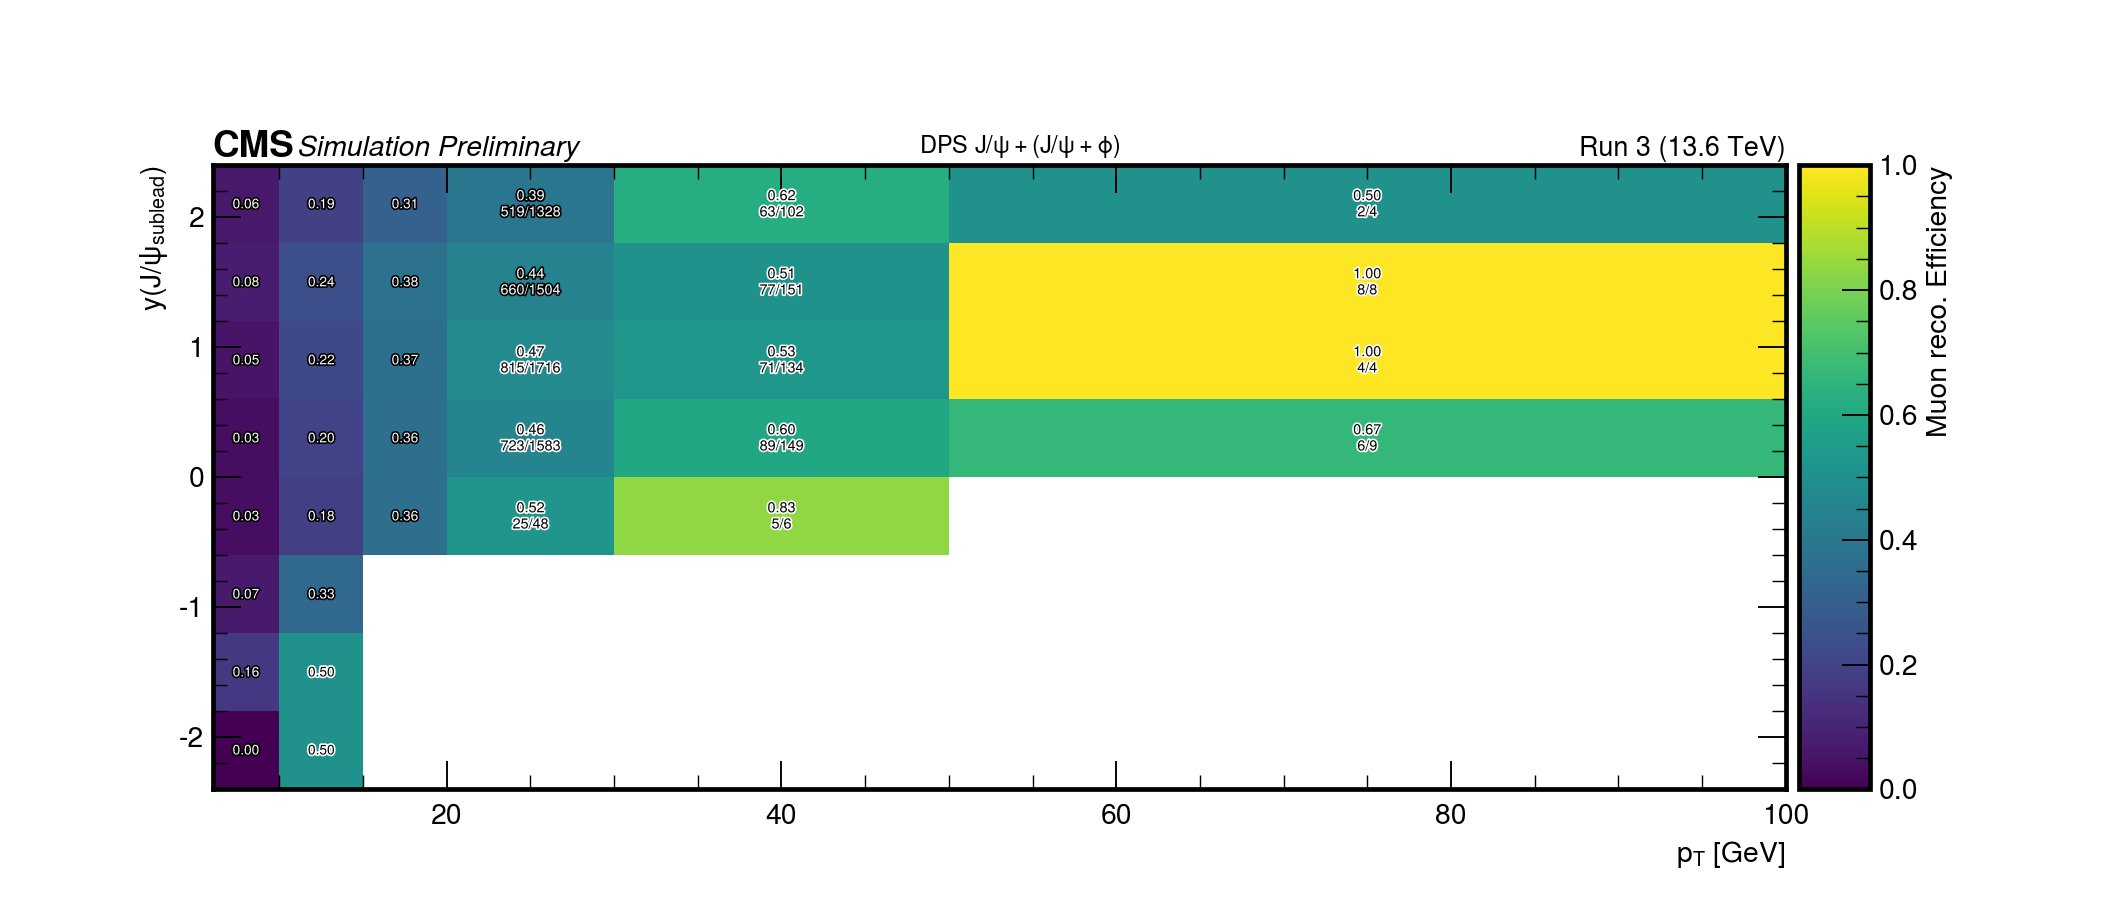
\includegraphics[width=0.85\textwidth]{figures/appendix-efficiency/object2d_jpsi_sublead_muonRECO.png}\\[2pt]
  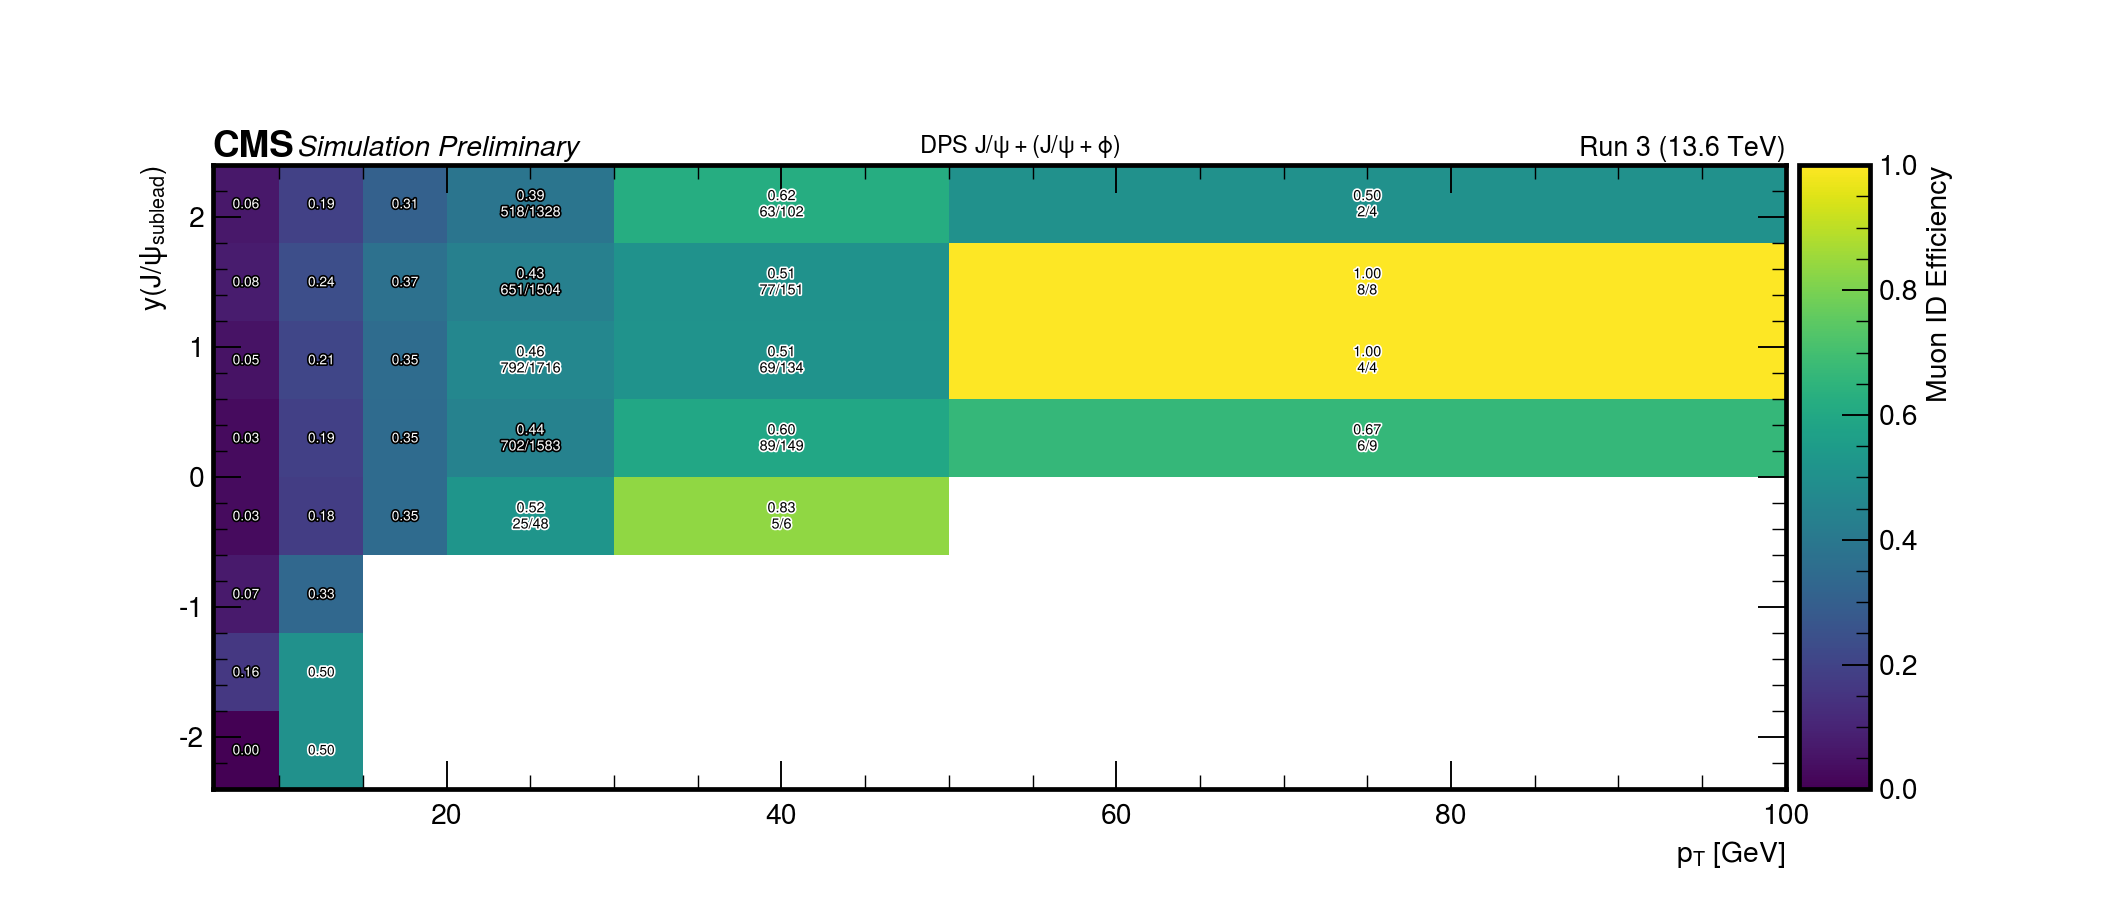
\includegraphics[width=0.85\textwidth]{figures/appendix-efficiency/object2d_jpsi_sublead_muonID.png}\\[2pt]
  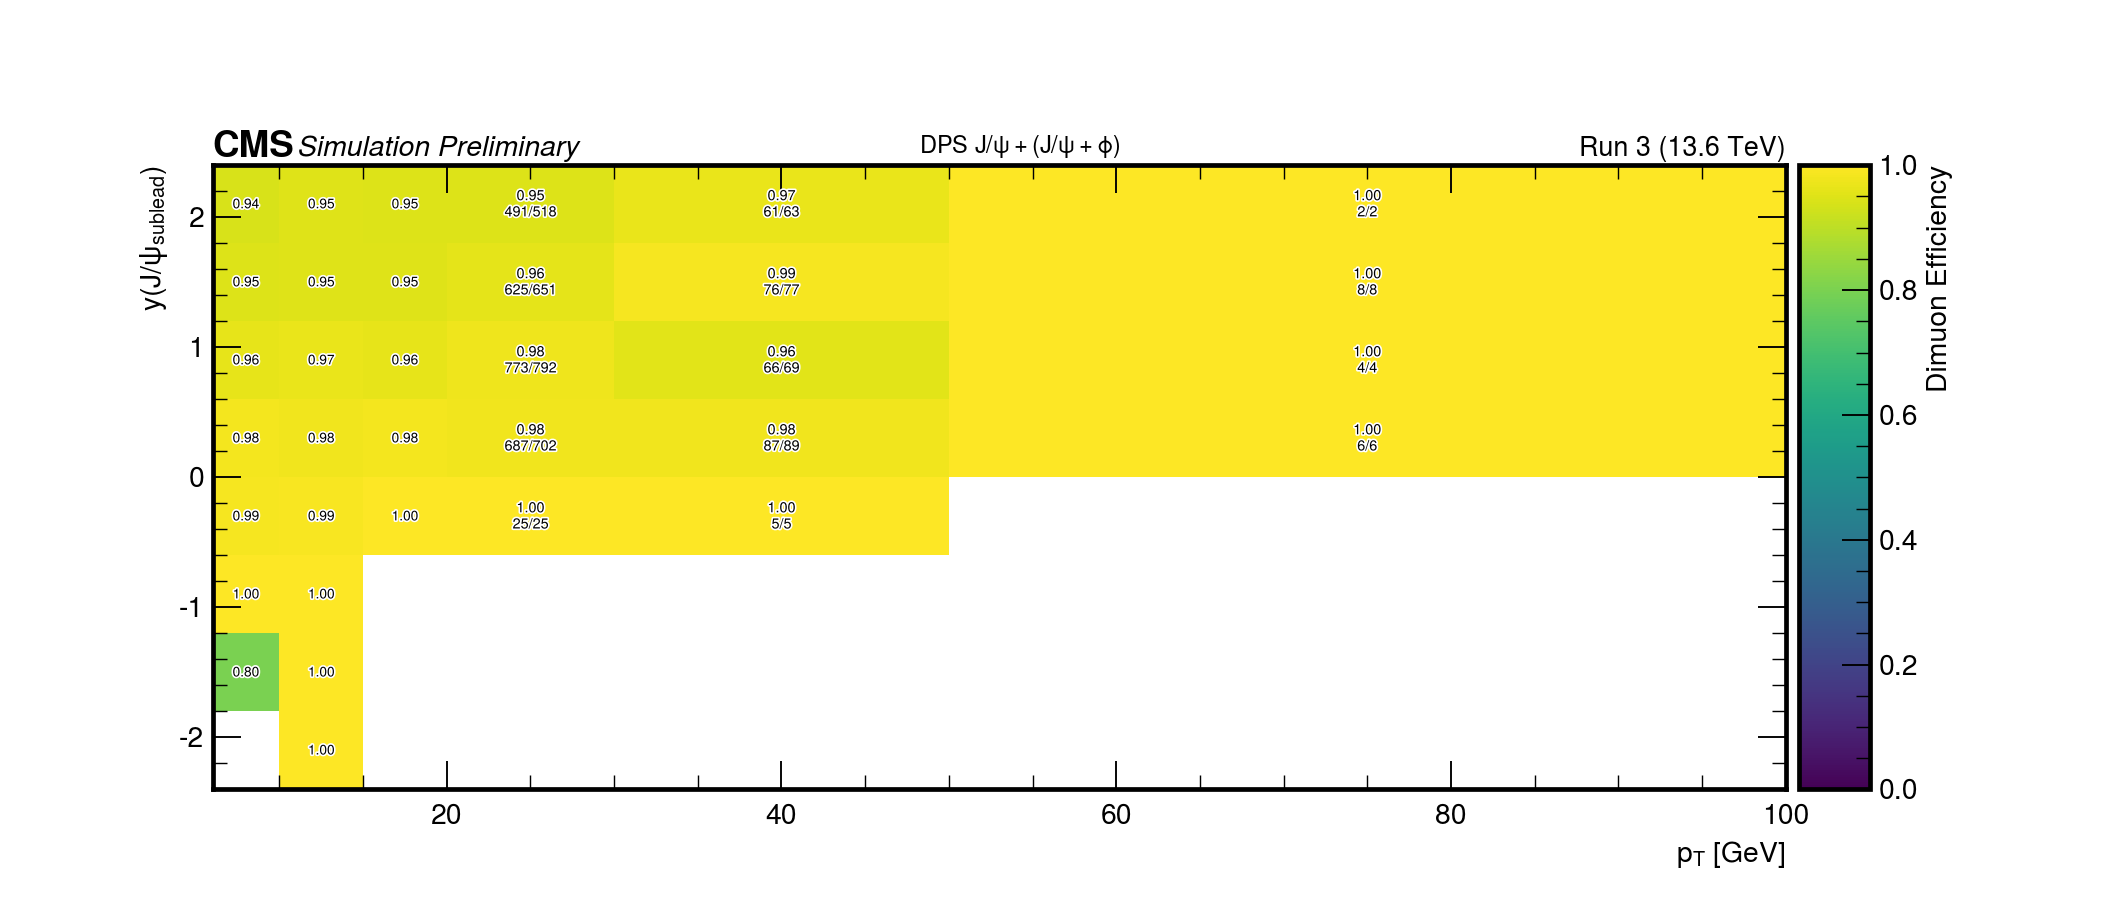
\includegraphics[width=0.85\textwidth]{figures/appendix-efficiency/object2d_jpsi_sublead_dimuon.png}
  \caption{Subleading $J/\psi$的条件效率（从上至下：缪子重建、缪子鉴别、双缪子选择）。}
  \label{fig:app-eff-jpsi-sublead}
\end{figure}

\begin{figure}[htbp]
  \centering
  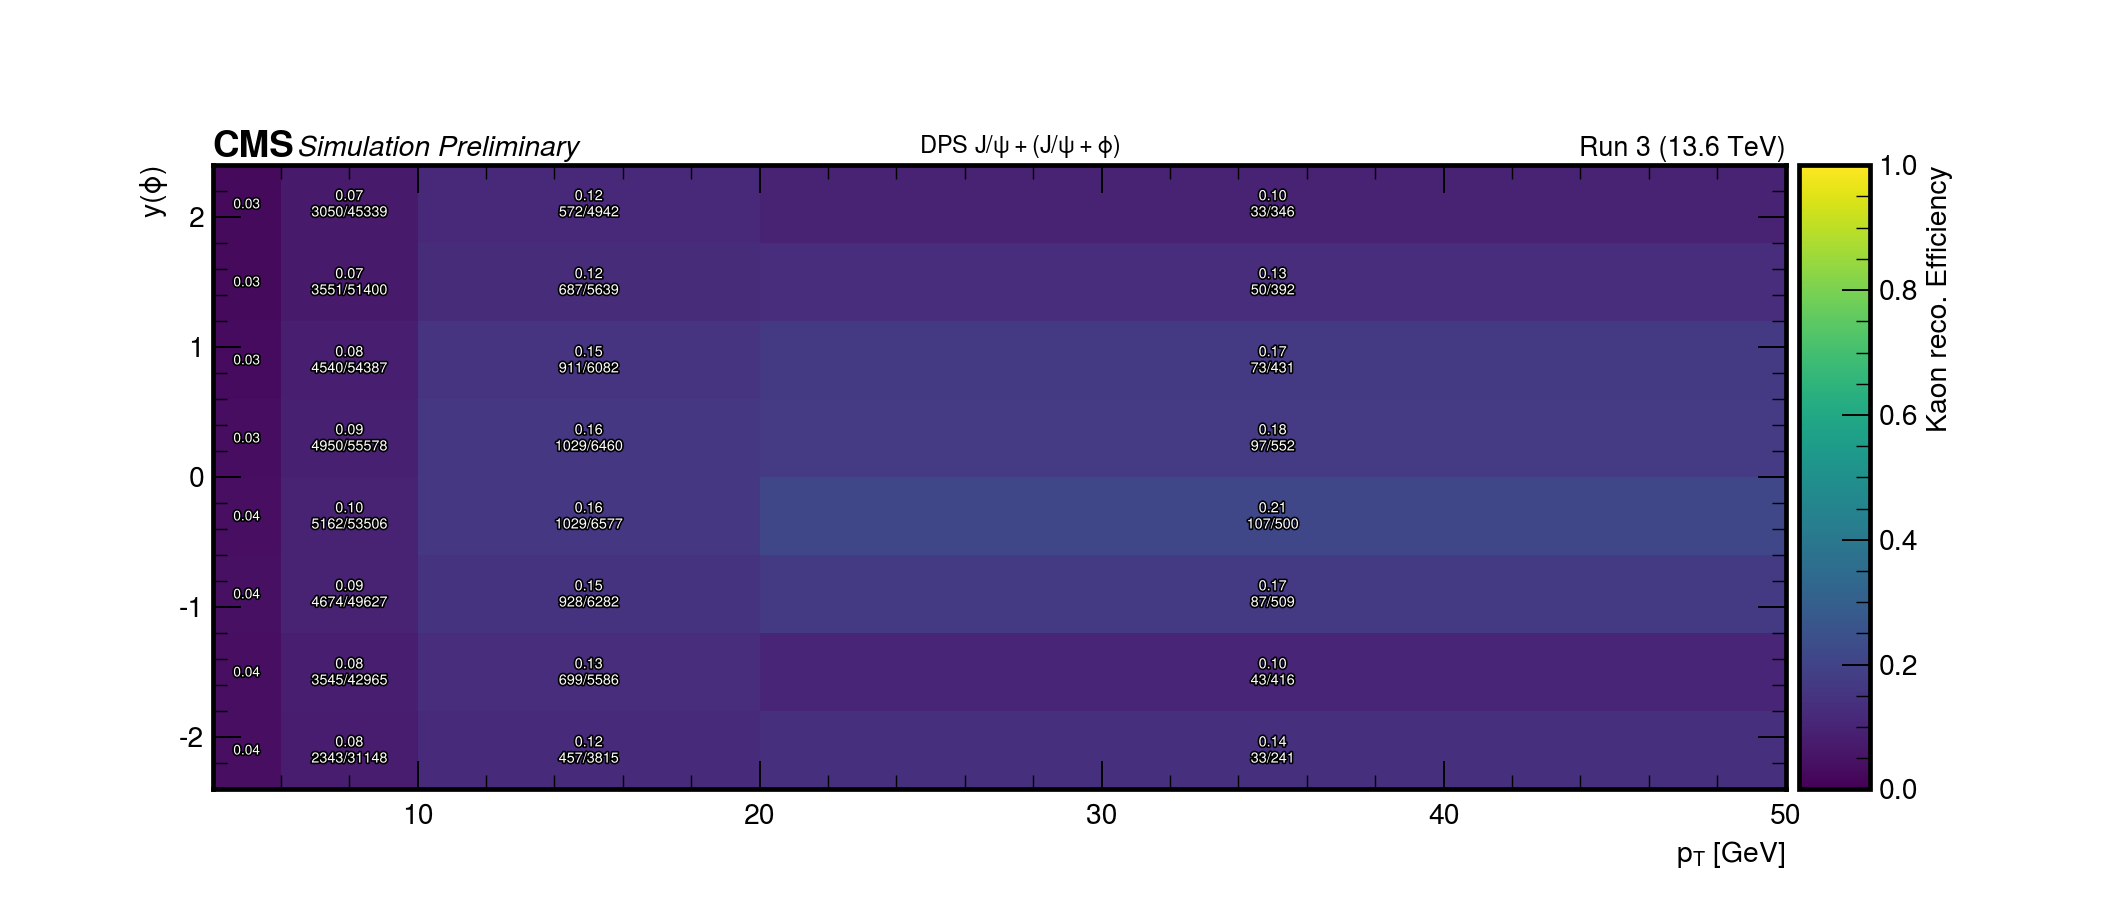
\includegraphics[width=0.85\textwidth]{figures/appendix-efficiency/object2d_phi_kaonRECO.png}\\[2pt]
  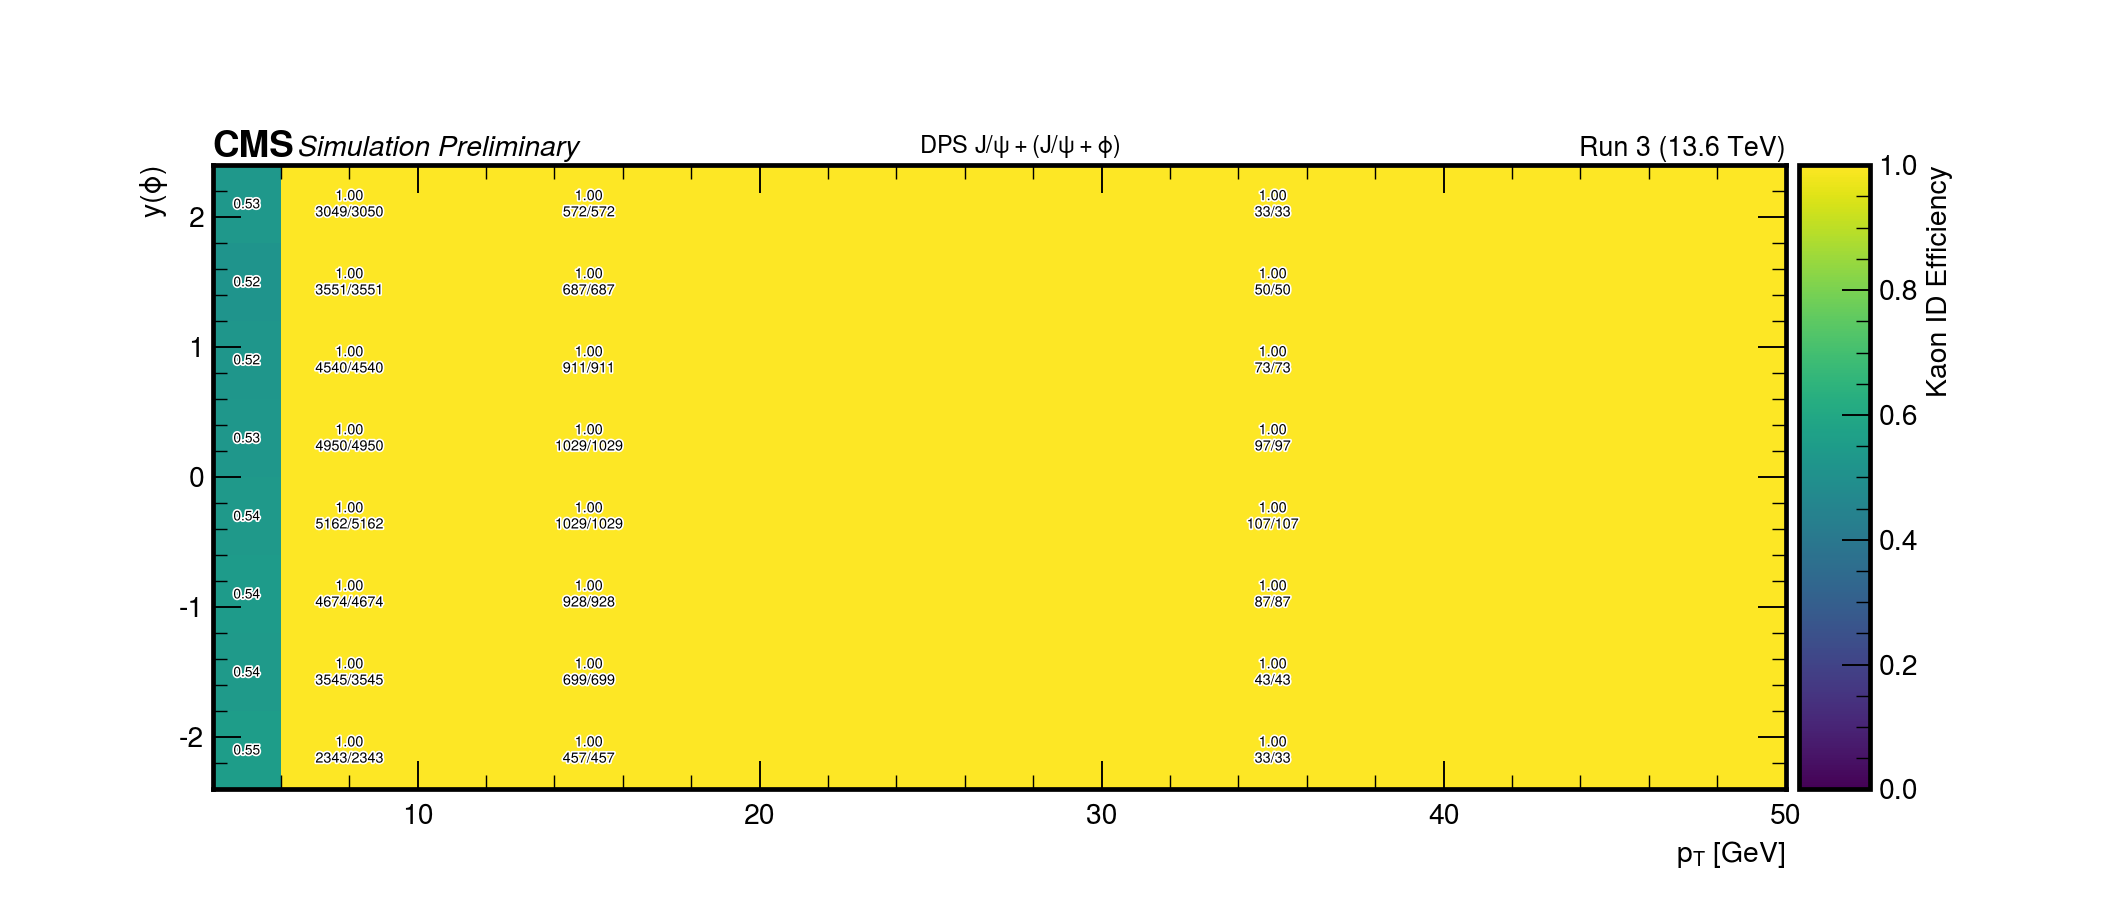
\includegraphics[width=0.85\textwidth]{figures/appendix-efficiency/object2d_phi_kaonID.png}\\[2pt]
  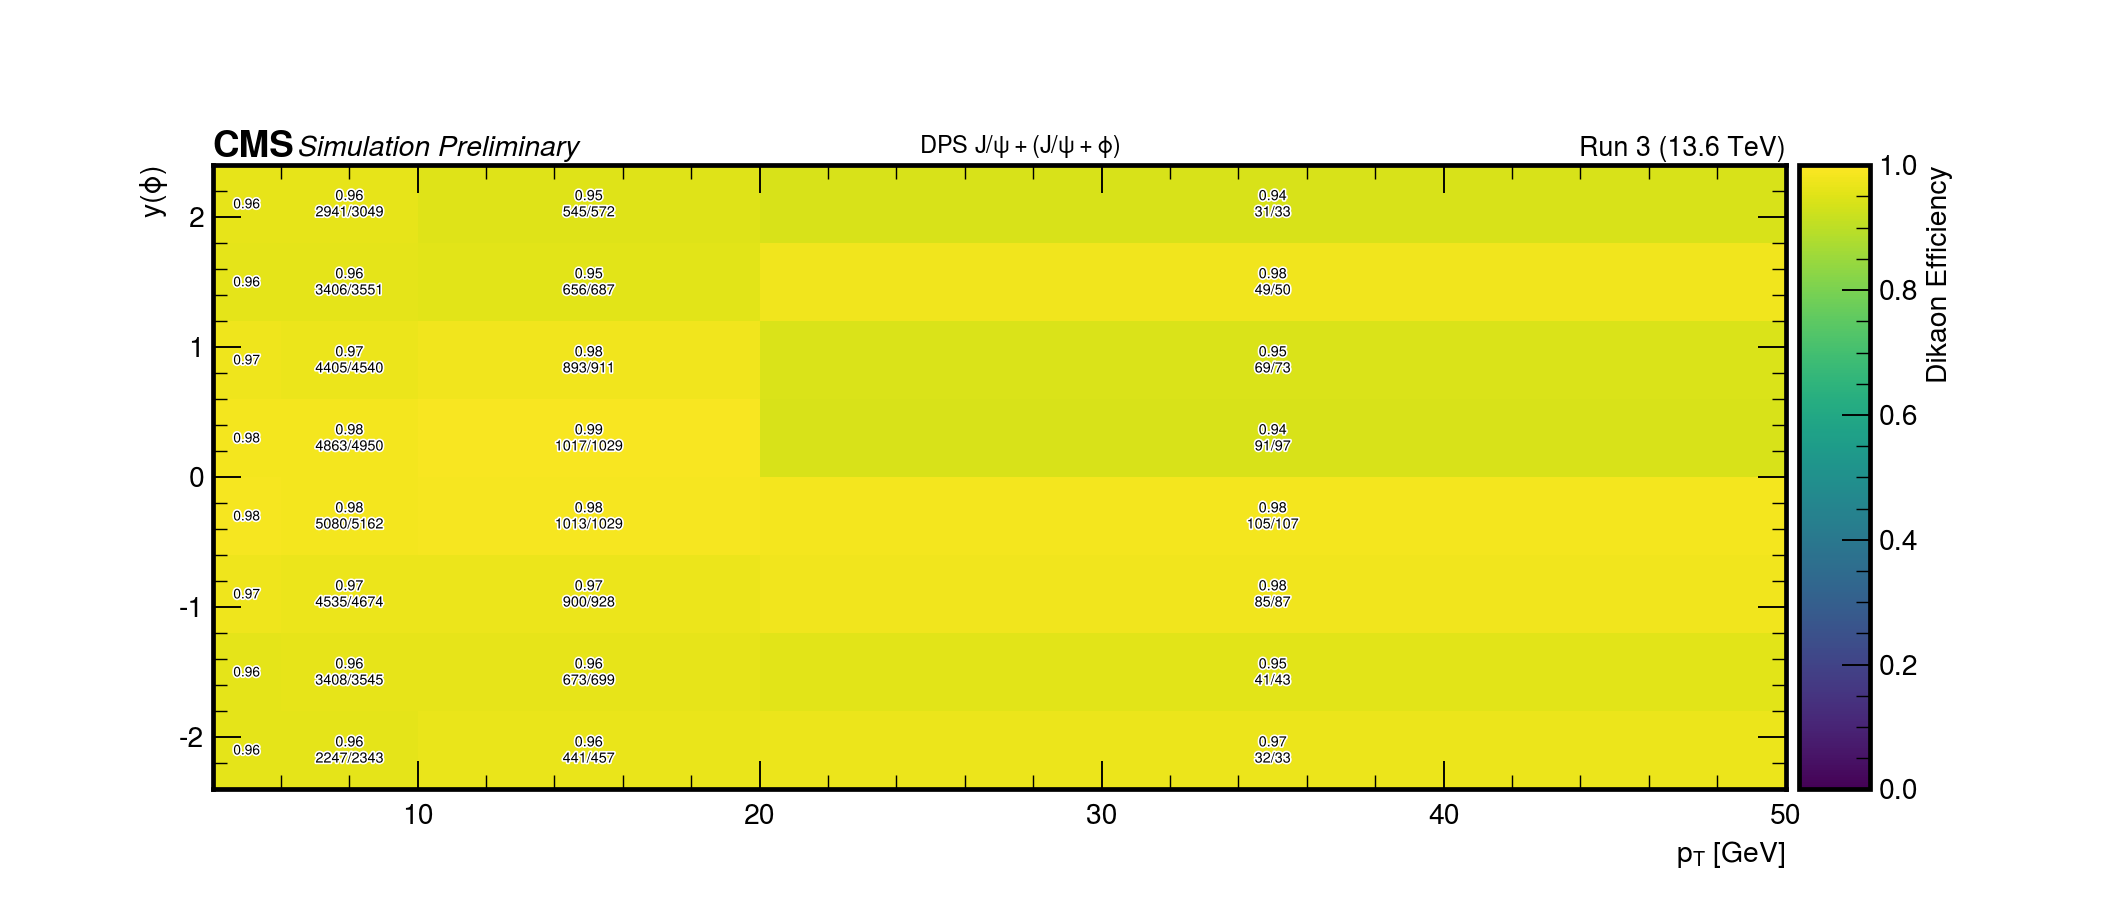
\includegraphics[width=0.85\textwidth]{figures/appendix-efficiency/object2d_phi_dikaon.png}
  \caption{$\phi$介子的条件效率（从上至下：介子重建、介子鉴别、双介子选择）。}
  \label{fig:app-eff-phi}
\end{figure}

\section{事例级效率}

\begin{figure}[htbp]
  \centering
  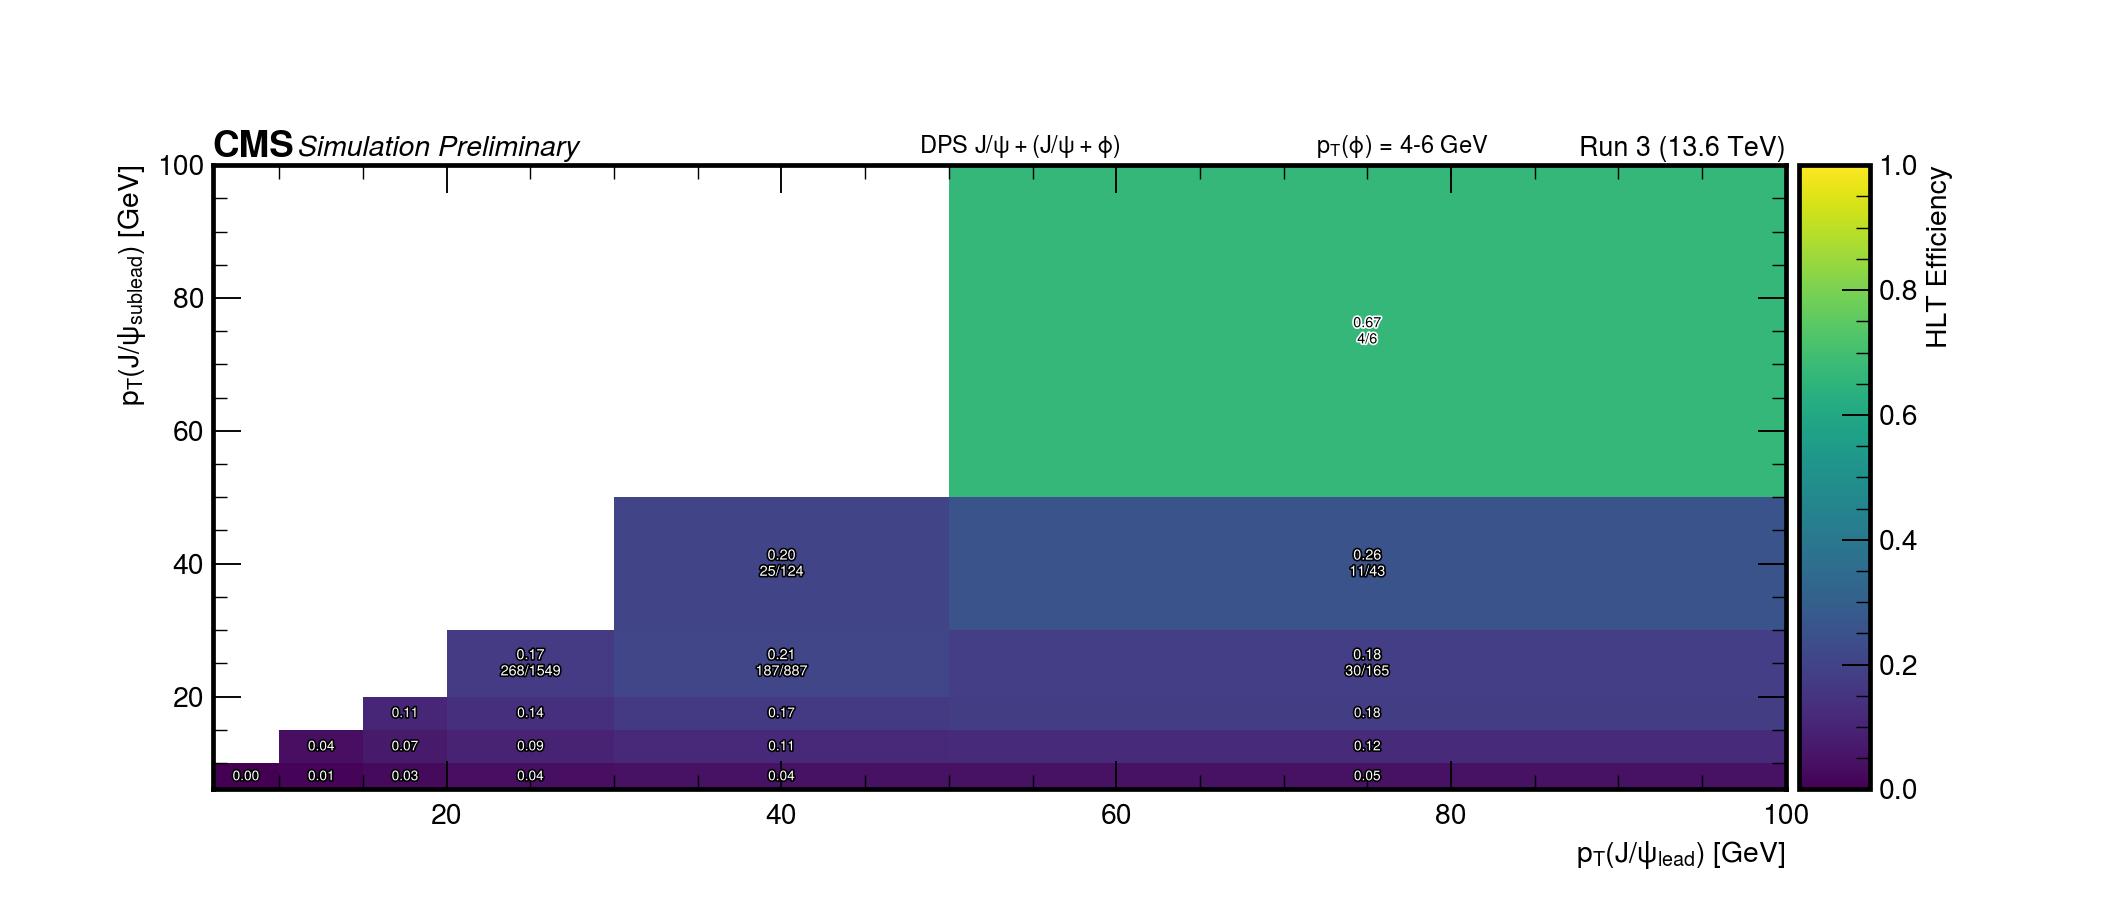
\includegraphics[width=0.85\textwidth]{figures/appendix-efficiency/corr3d_hlt_event_phiPt_0.0.png}\\[2pt]
  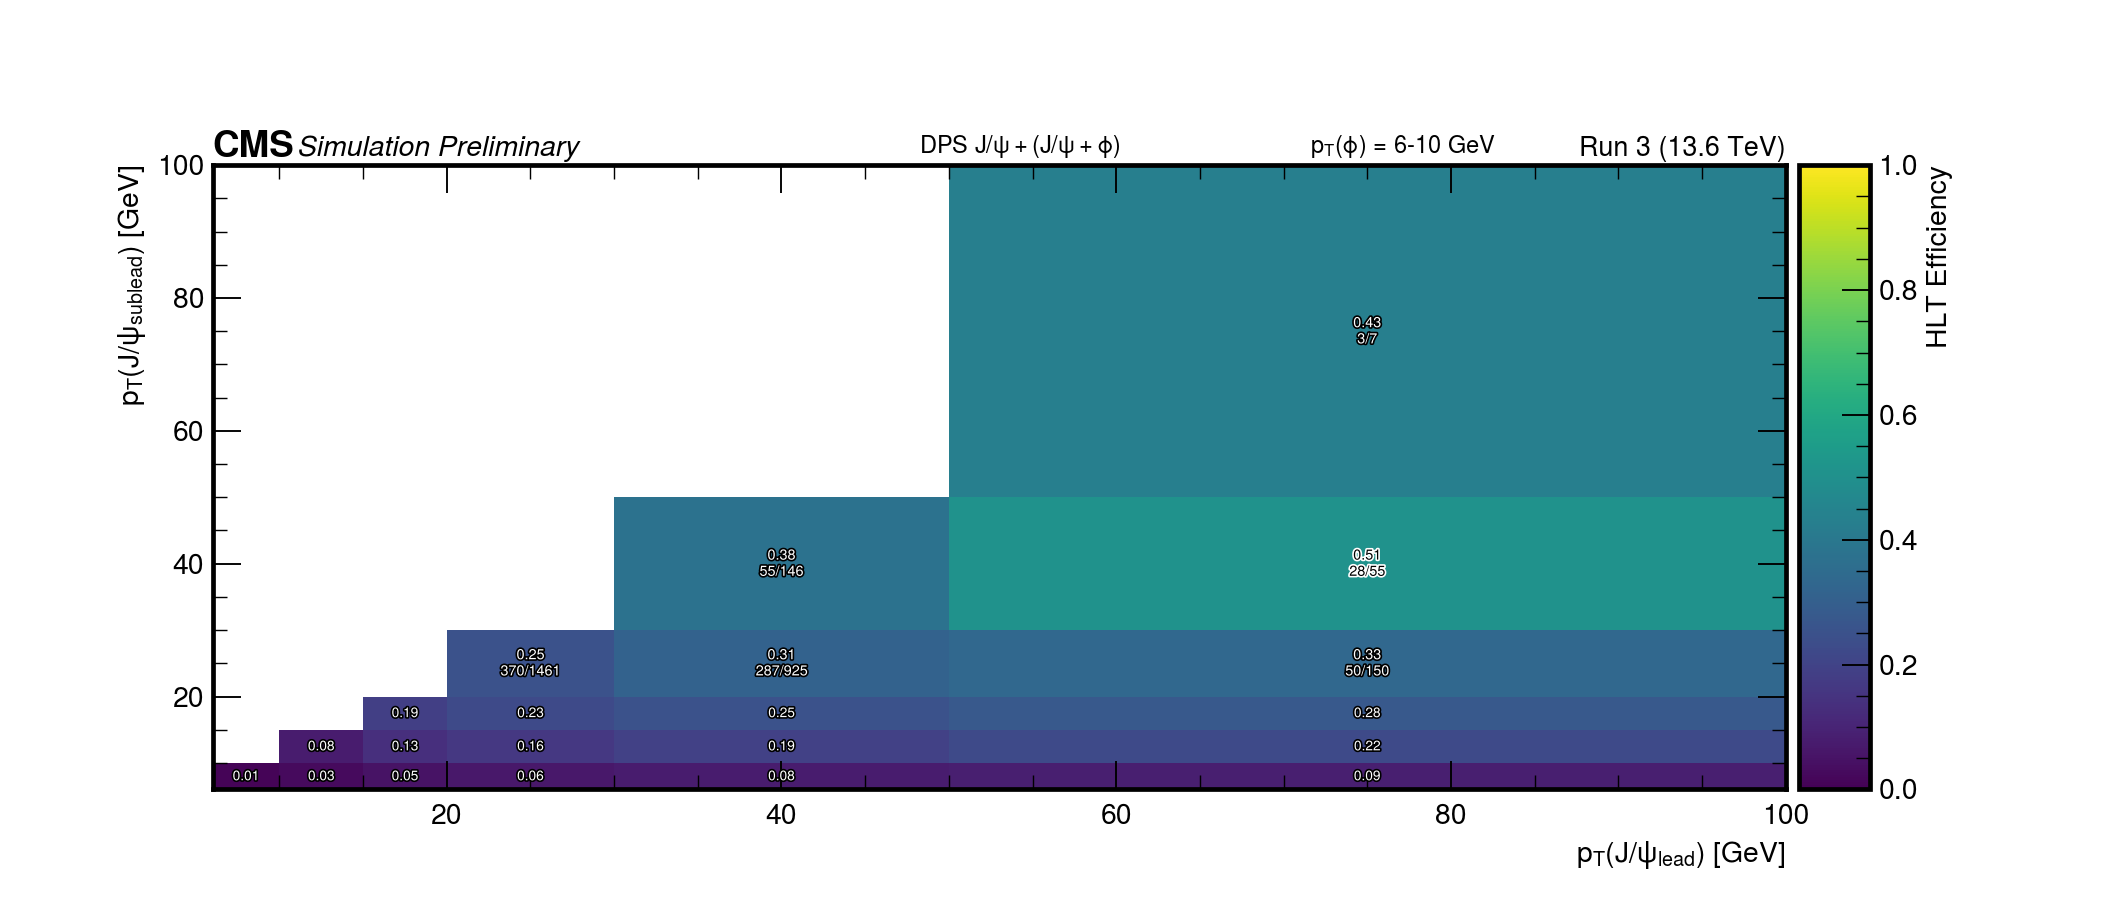
\includegraphics[width=0.85\textwidth]{figures/appendix-efficiency/corr3d_hlt_event_phiPt_1.0.png}\\[2pt]
  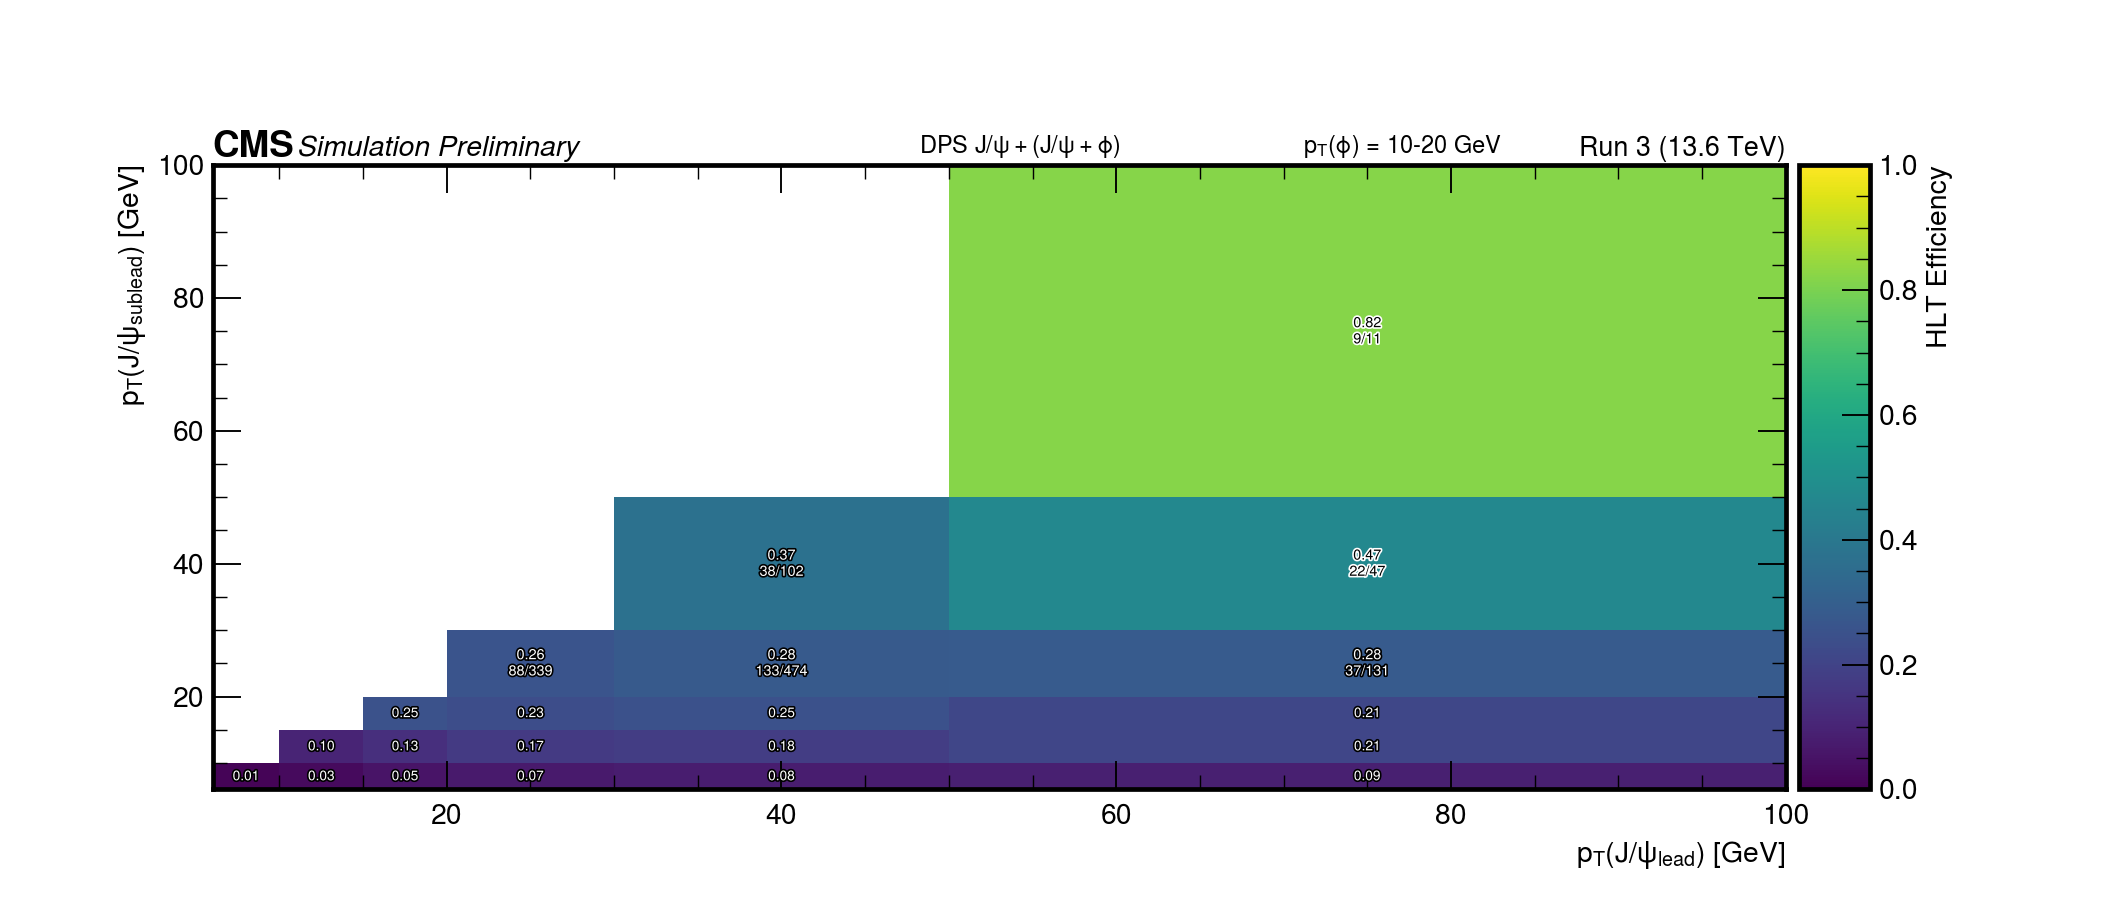
\includegraphics[width=0.85\textwidth]{figures/appendix-efficiency/corr3d_hlt_event_phiPt_2.0.png}\\[2pt]
  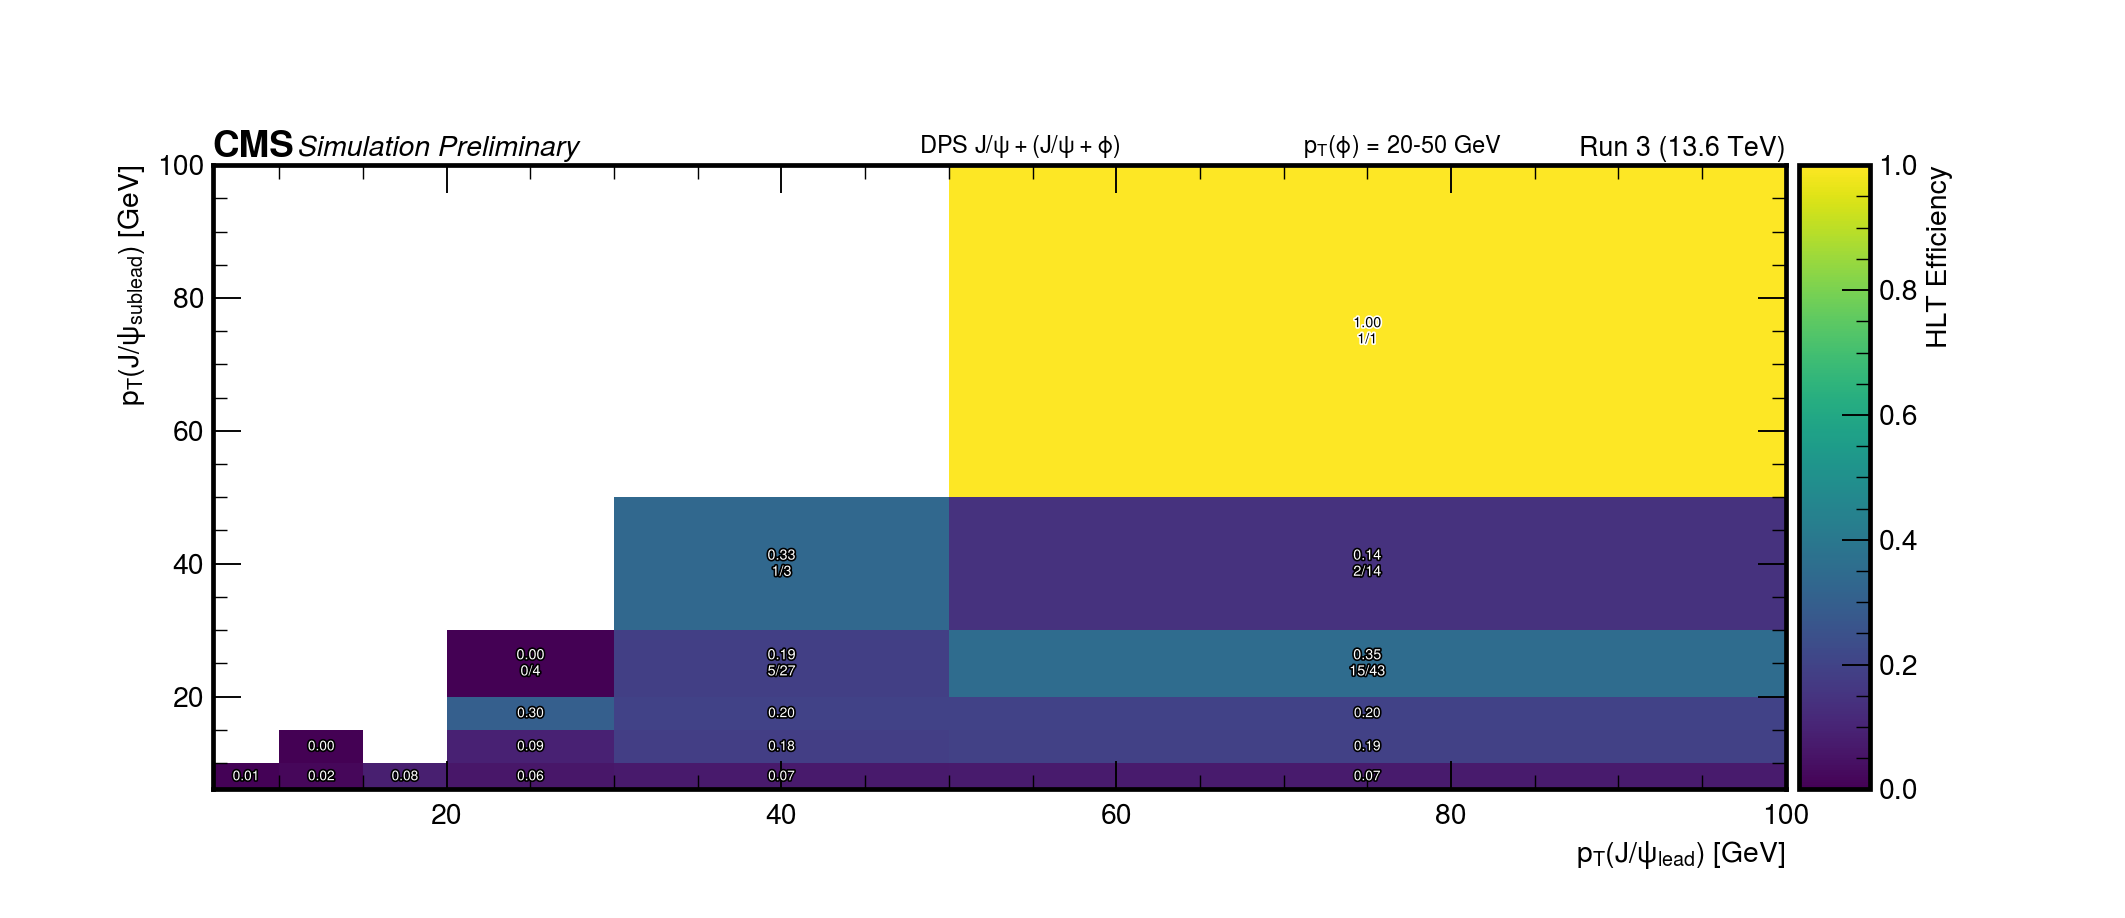
\includegraphics[width=0.85\textwidth]{figures/appendix-efficiency/corr3d_hlt_event_phiPt_3.0.png}
  \caption{HLT触发效率作为$p_{\mathrm{T}}(J/\psi_1)$和$p_{\mathrm{T}}(J/\psi_2)$的函数，按$p_{\mathrm{T}}(\phi)$区间从上至下：\SIrange{4}{6}{\giga\eV}、\SIrange{6}{10}{\giga\eV}、\SIrange{10}{20}{\giga\eV}、\SIrange{20}{50}{\giga\eV}。}
  \label{fig:app-eff-hlt}
\end{figure}

\begin{figure}[htbp]
  \centering
  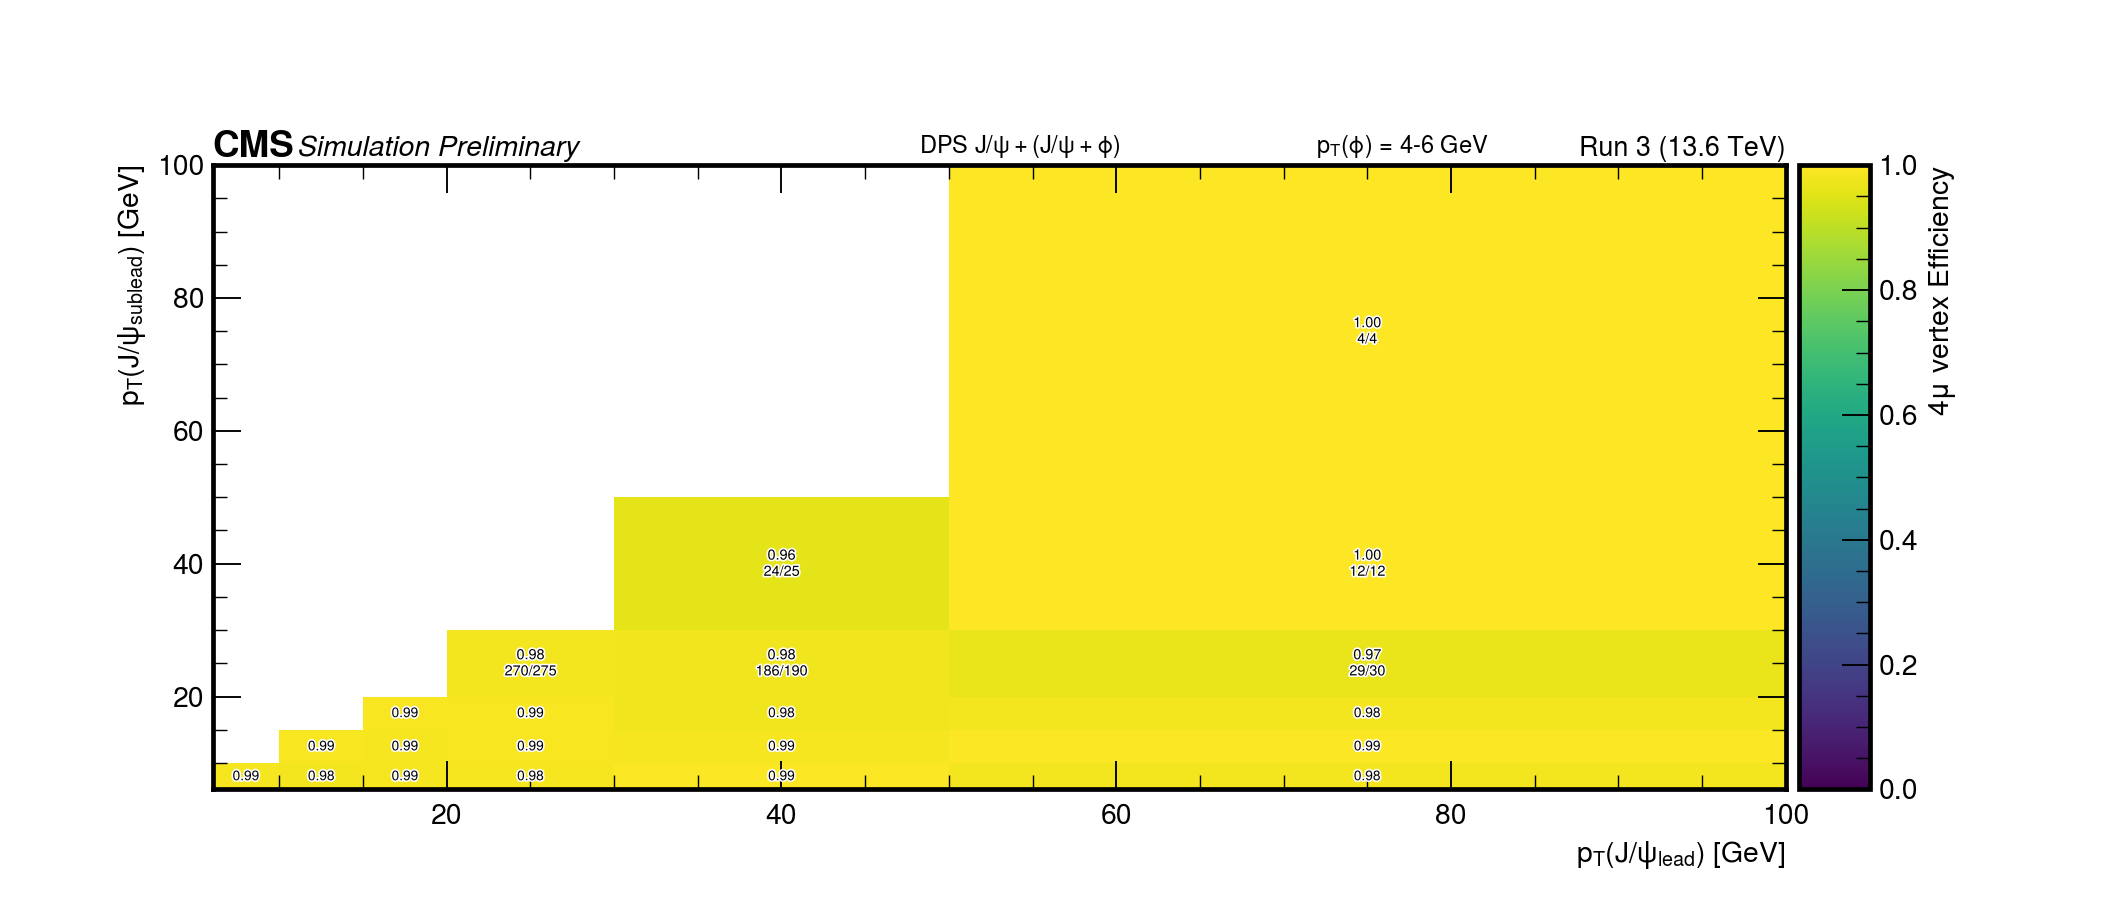
\includegraphics[width=0.85\textwidth]{figures/appendix-efficiency/corr3d_four_muon_vtx_phiPt_0.0.png}\\[2pt]
  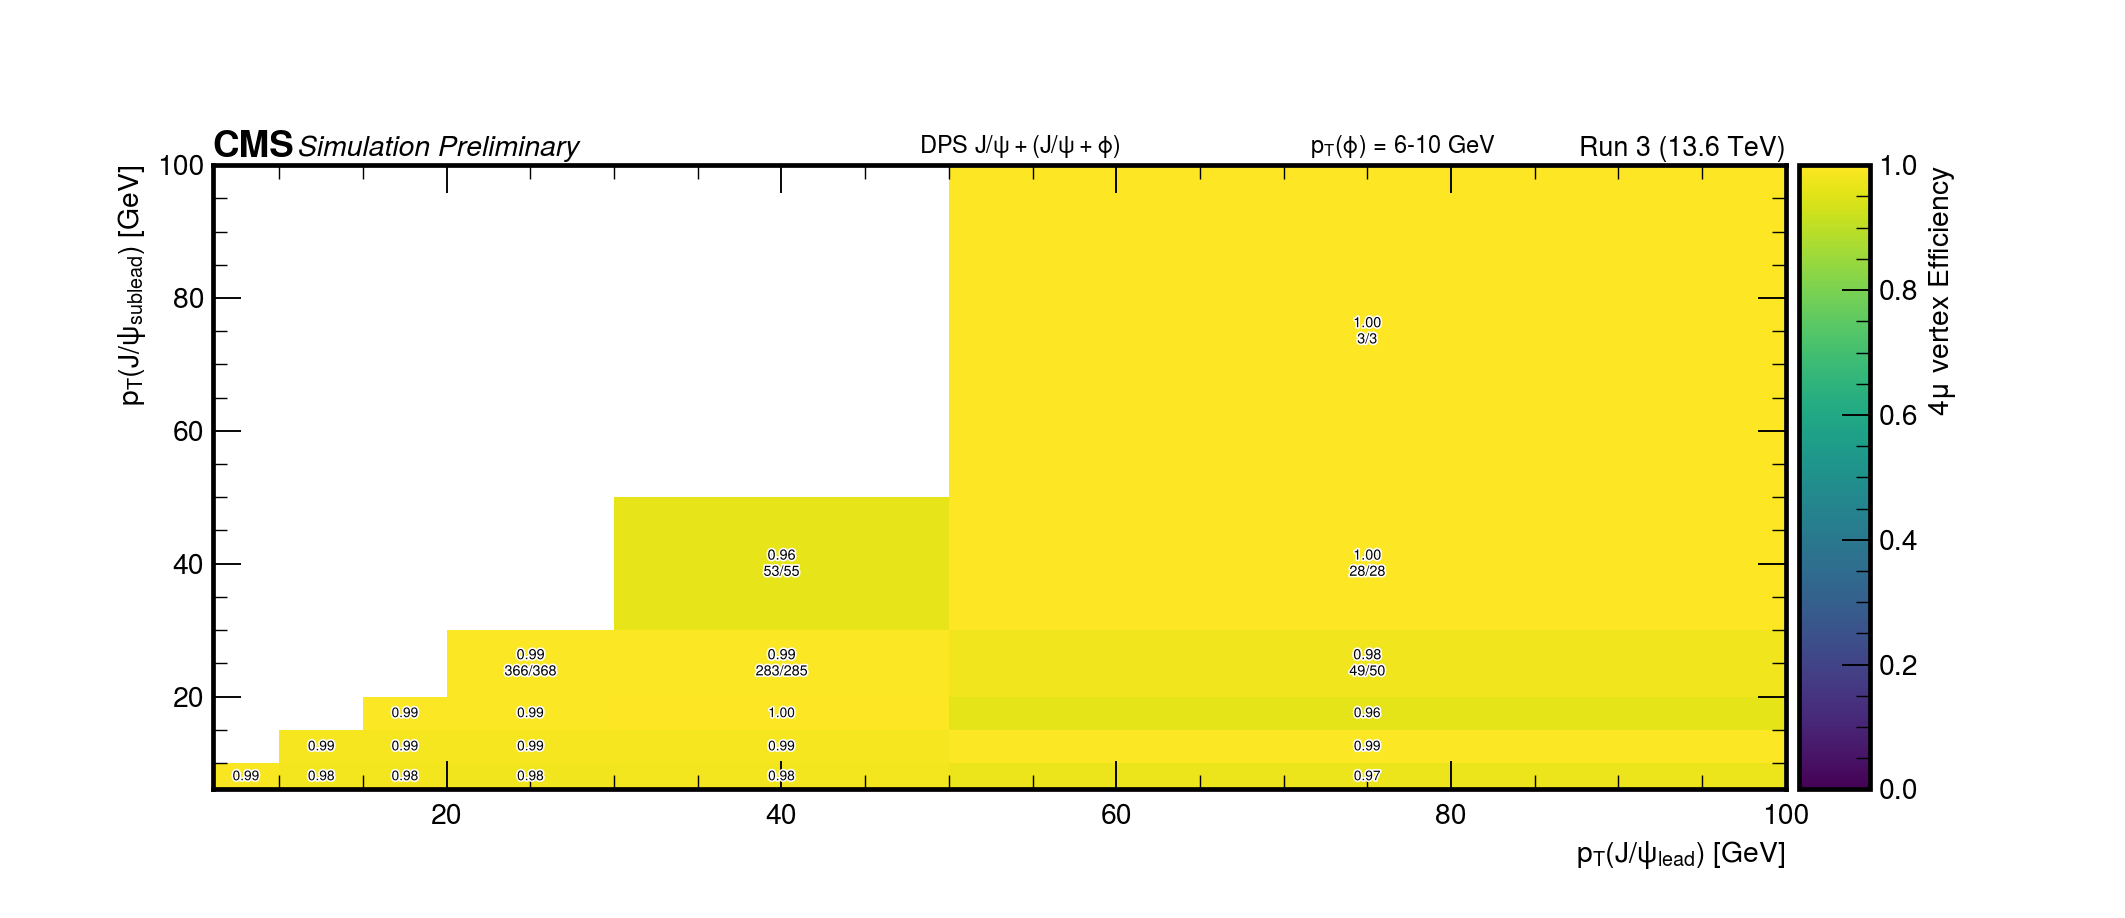
\includegraphics[width=0.85\textwidth]{figures/appendix-efficiency/corr3d_four_muon_vtx_phiPt_1.0.png}\\[2pt]
  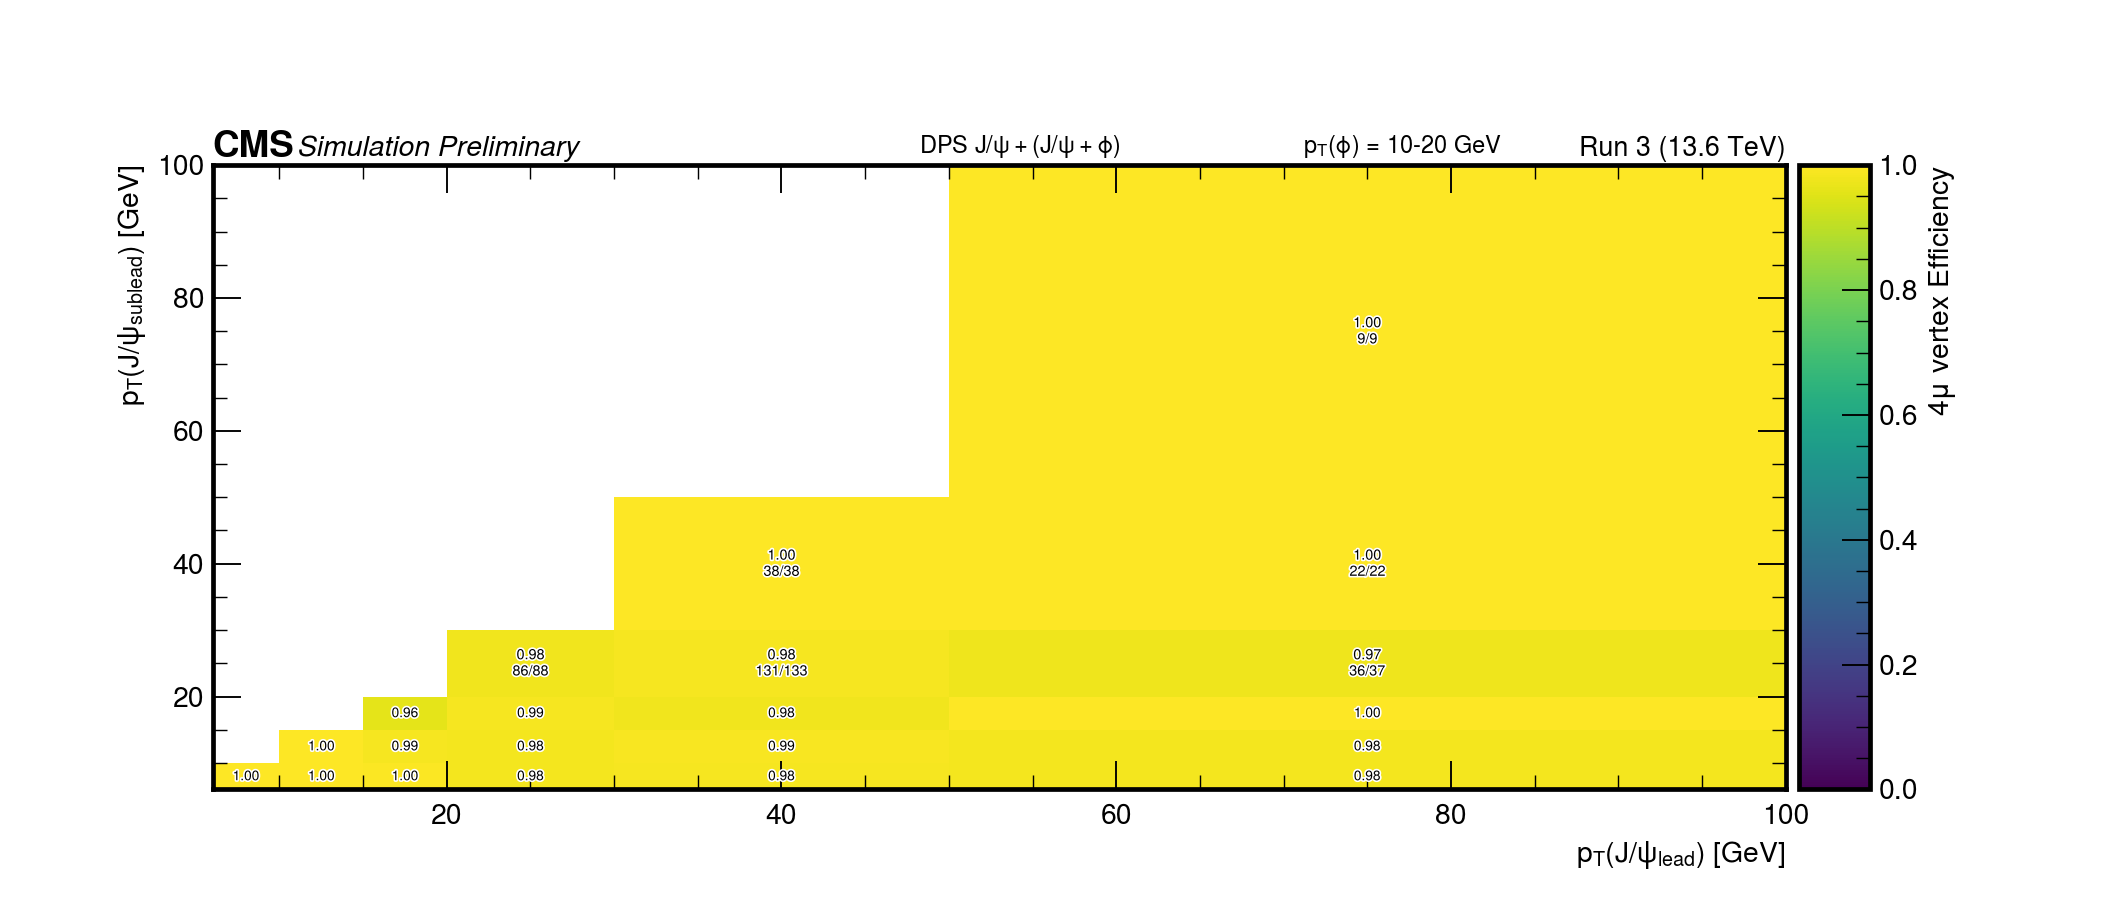
\includegraphics[width=0.85\textwidth]{figures/appendix-efficiency/corr3d_four_muon_vtx_phiPt_2.0.png}\\[2pt]
  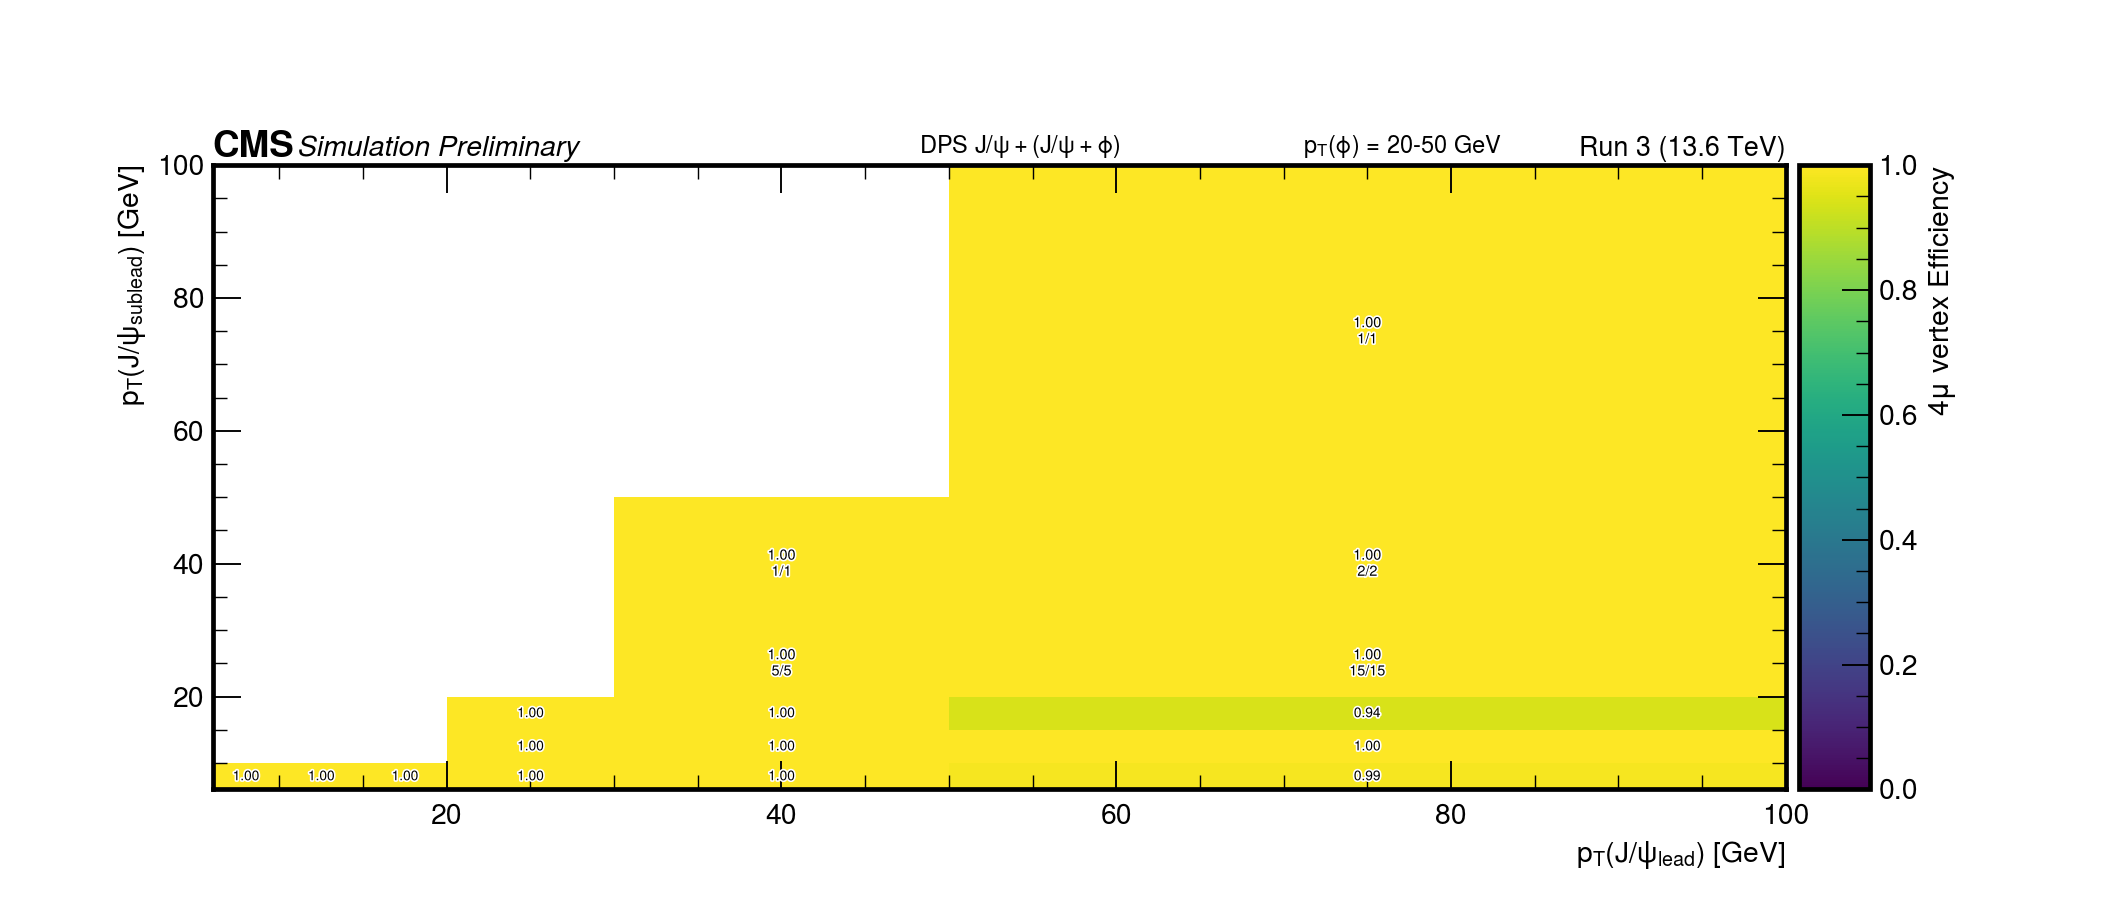
\includegraphics[width=0.85\textwidth]{figures/appendix-efficiency/corr3d_four_muon_vtx_phiPt_3.0.png}
  \caption{四缪子顶点效率作为$p_{\mathrm{T}}(J/\psi_1)$和$p_{\mathrm{T}}(J/\psi_2)$的函数，按$p_{\mathrm{T}}(\phi)$区间分组，同图~\ref{fig:app-eff-hlt}。}
  \label{fig:app-eff-fourmu-vtx}
\end{figure}

\begin{figure}[htbp]
  \centering
  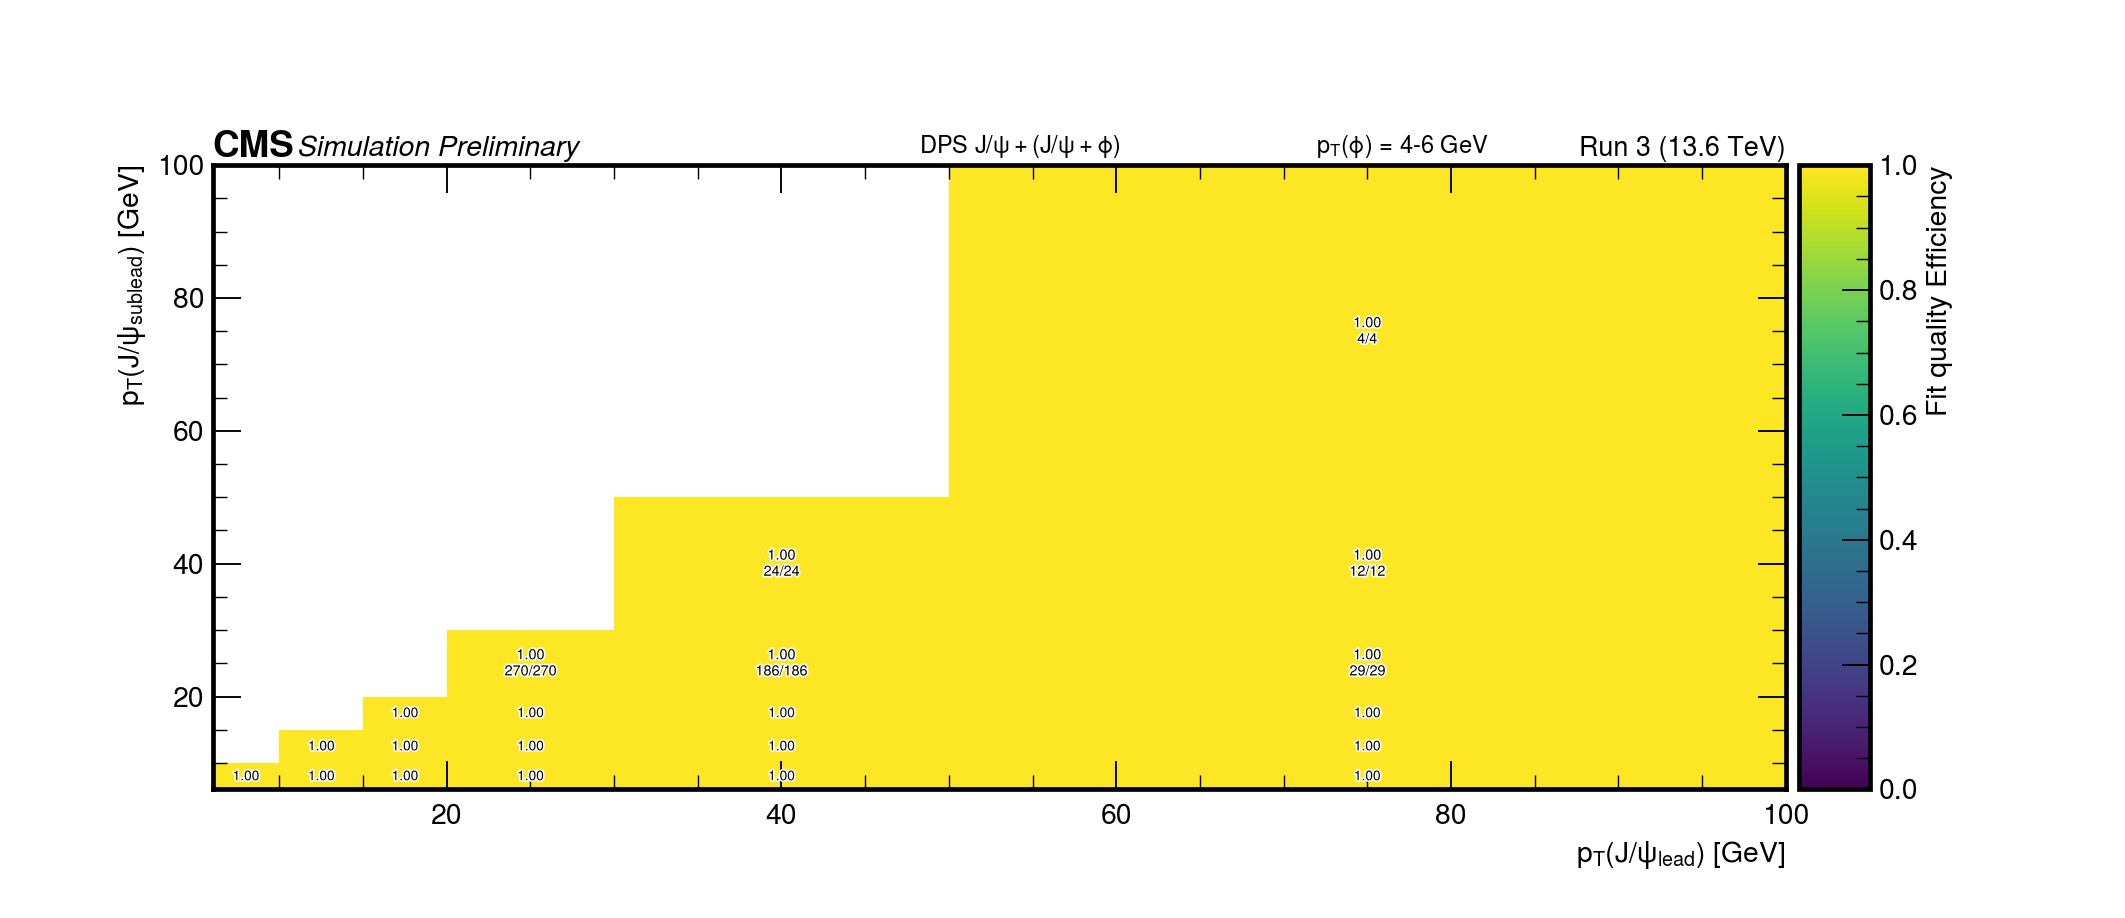
\includegraphics[width=0.85\textwidth]{figures/appendix-efficiency/corr3d_Pri_fitPass_phiPt_0.0.png}\\[2pt]
  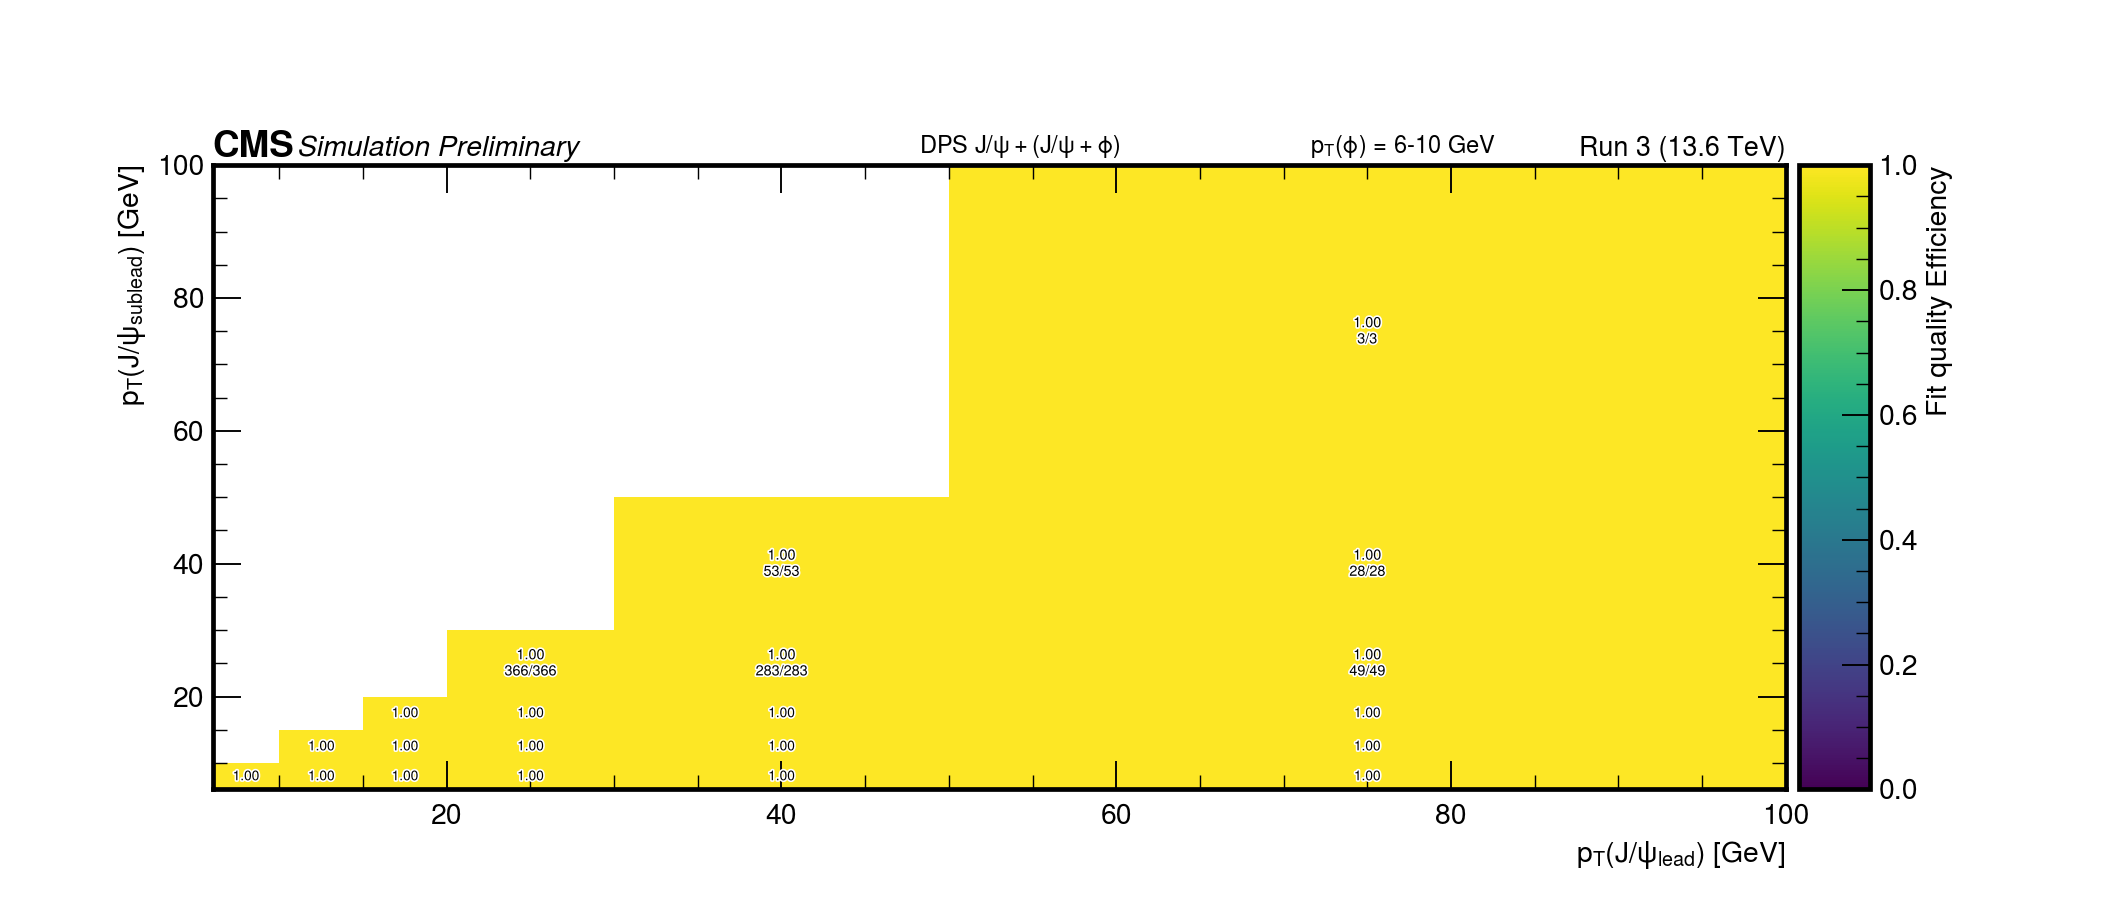
\includegraphics[width=0.85\textwidth]{figures/appendix-efficiency/corr3d_Pri_fitPass_phiPt_1.0.png}\\[2pt]
  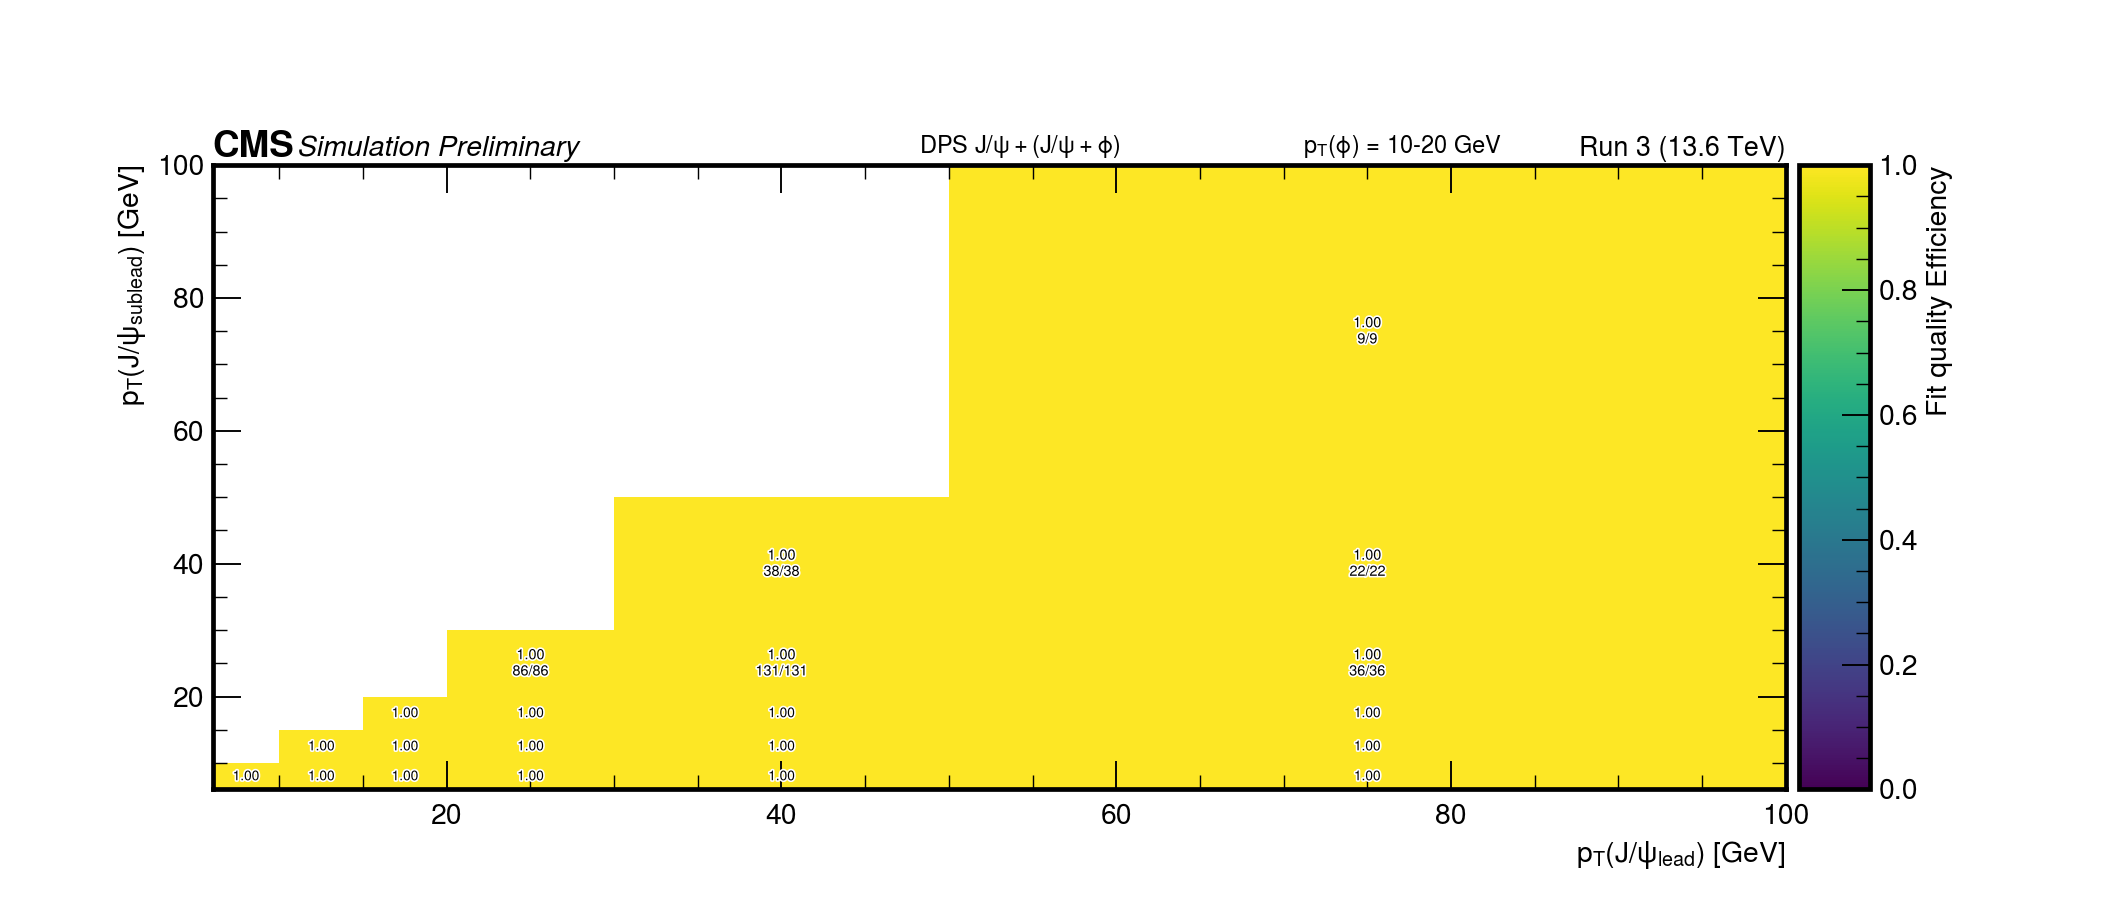
\includegraphics[width=0.85\textwidth]{figures/appendix-efficiency/corr3d_Pri_fitPass_phiPt_2.0.png}\\[2pt]
  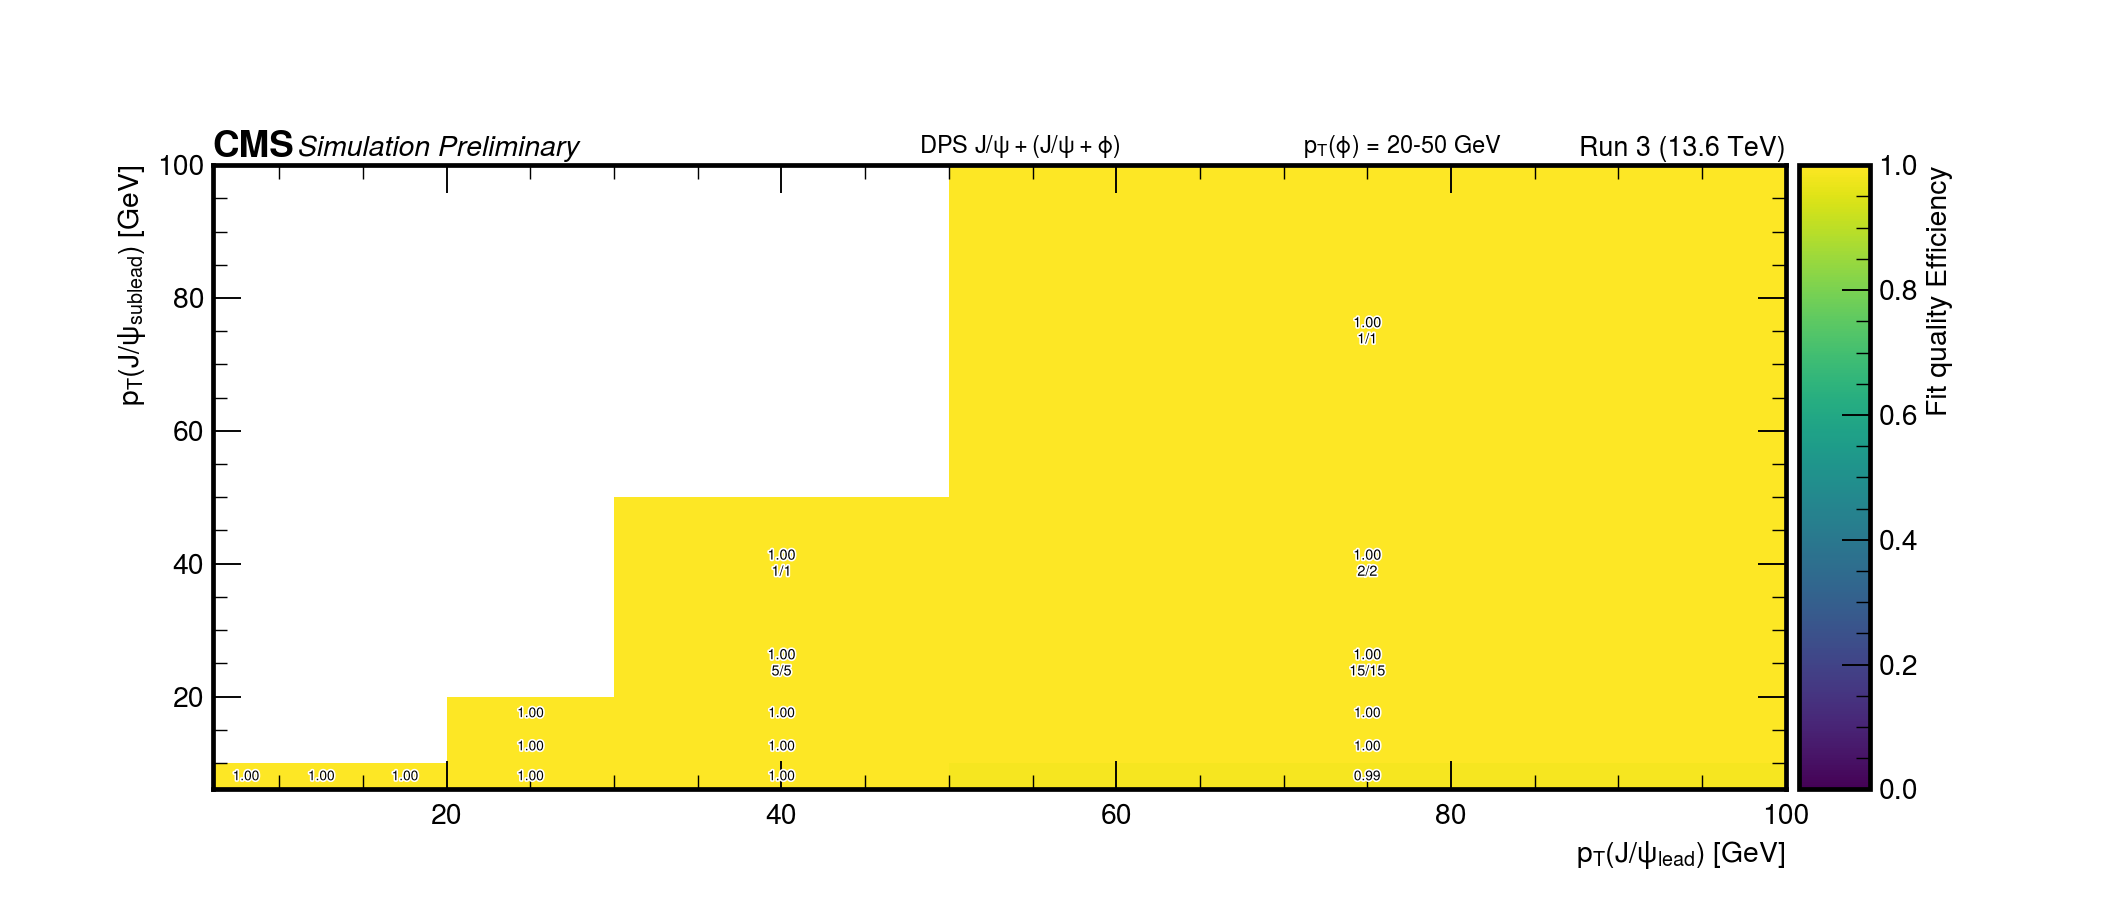
\includegraphics[width=0.85\textwidth]{figures/appendix-efficiency/corr3d_Pri_fitPass_phiPt_3.0.png}
  \caption{初级顶点拟合通过效率（$\epsilon_{\mathrm{Pri\_fitPass}}$）作为$p_{\mathrm{T}}(J/\psi_1)$和$p_{\mathrm{T}}(J/\psi_2)$的函数，按$p_{\mathrm{T}}(\phi)$区间分组。}
  \label{fig:app-eff-pri-fitpass}
\end{figure}

\begin{figure}[htbp]
  \centering
  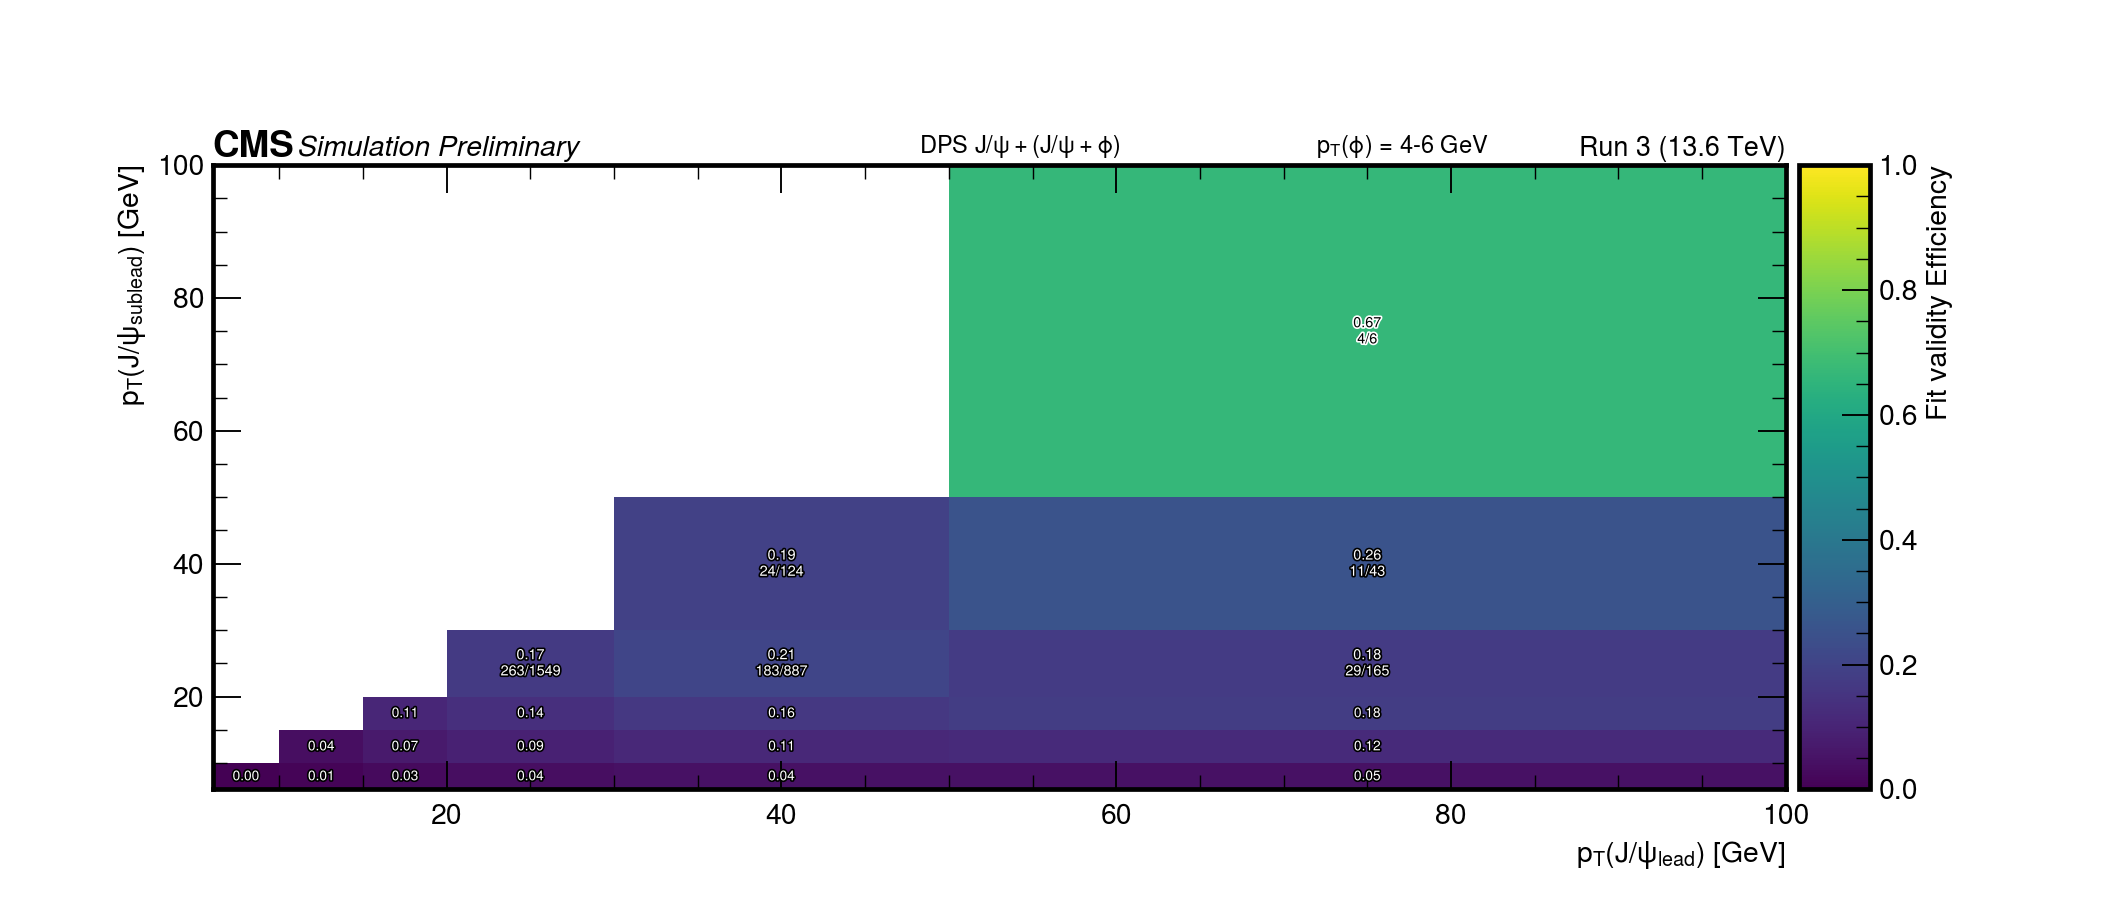
\includegraphics[width=0.85\textwidth]{figures/appendix-efficiency/corr3d_Pri_fitValid_phiPt_0.0.png}\\[2pt]
  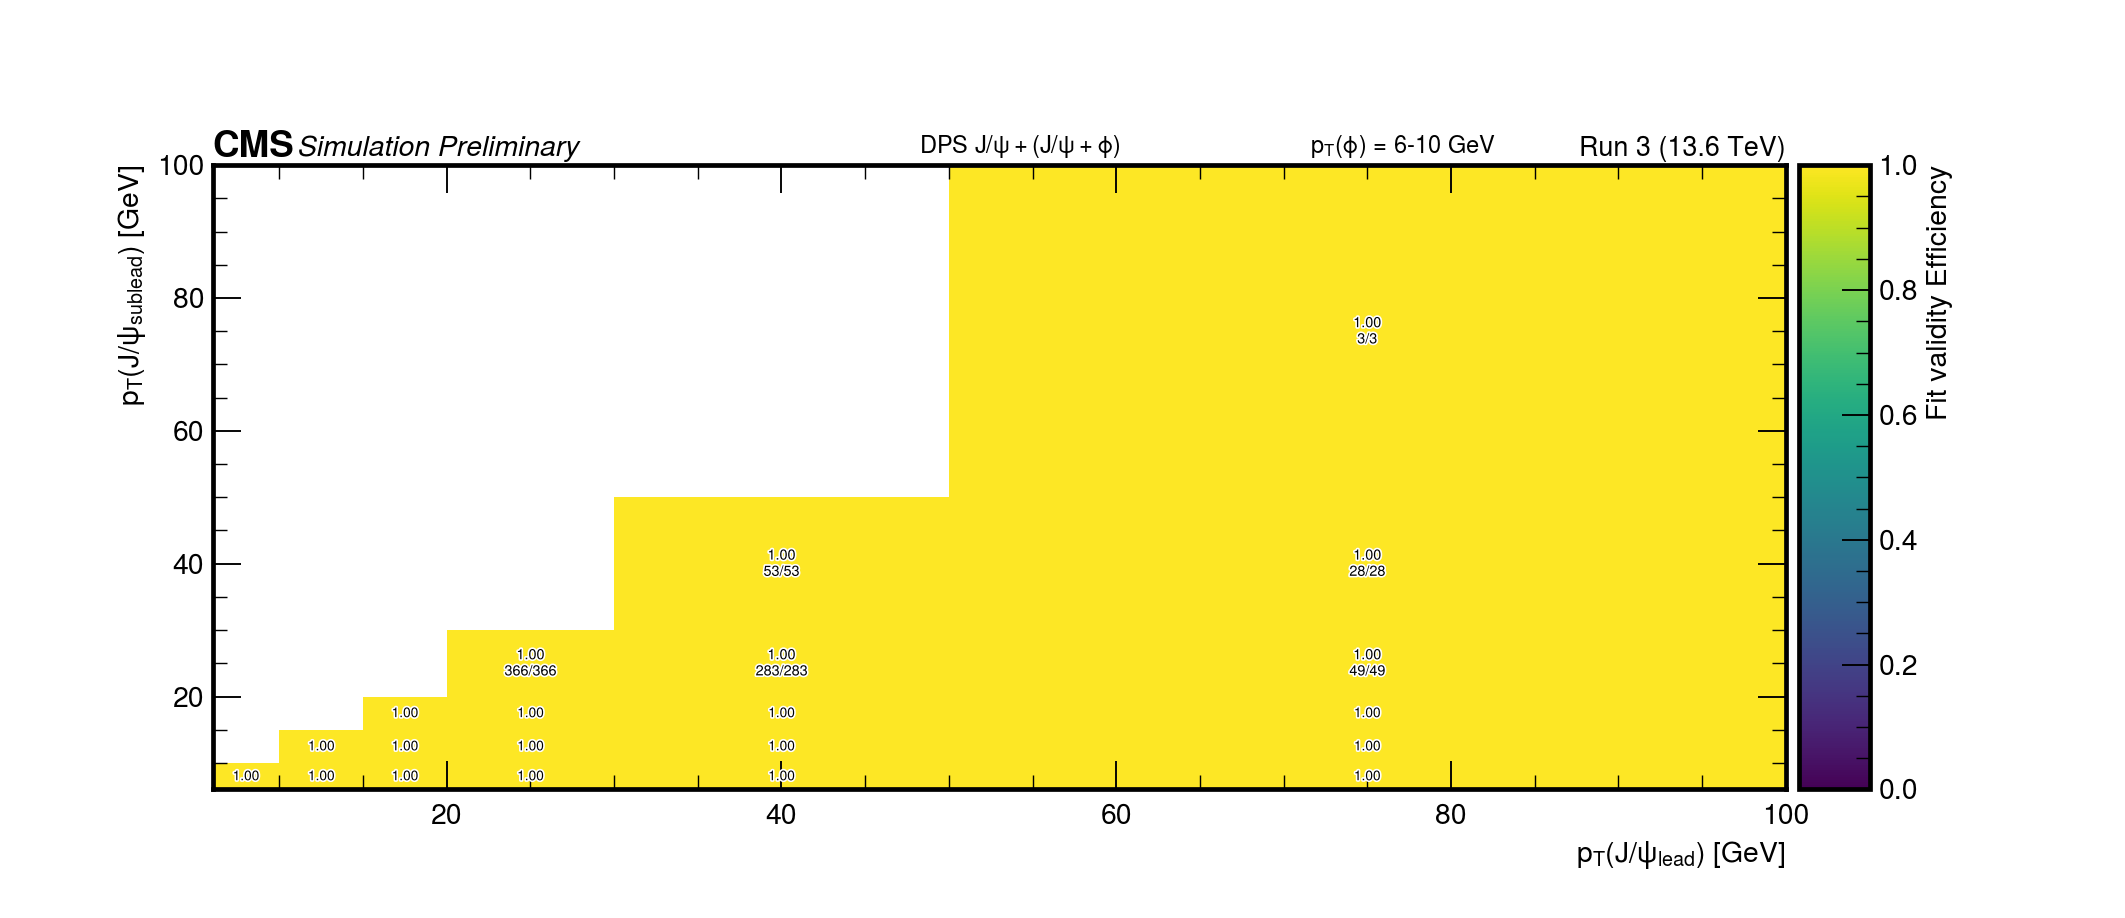
\includegraphics[width=0.85\textwidth]{figures/appendix-efficiency/corr3d_Pri_fitValid_phiPt_1.0.png}\\[2pt]
  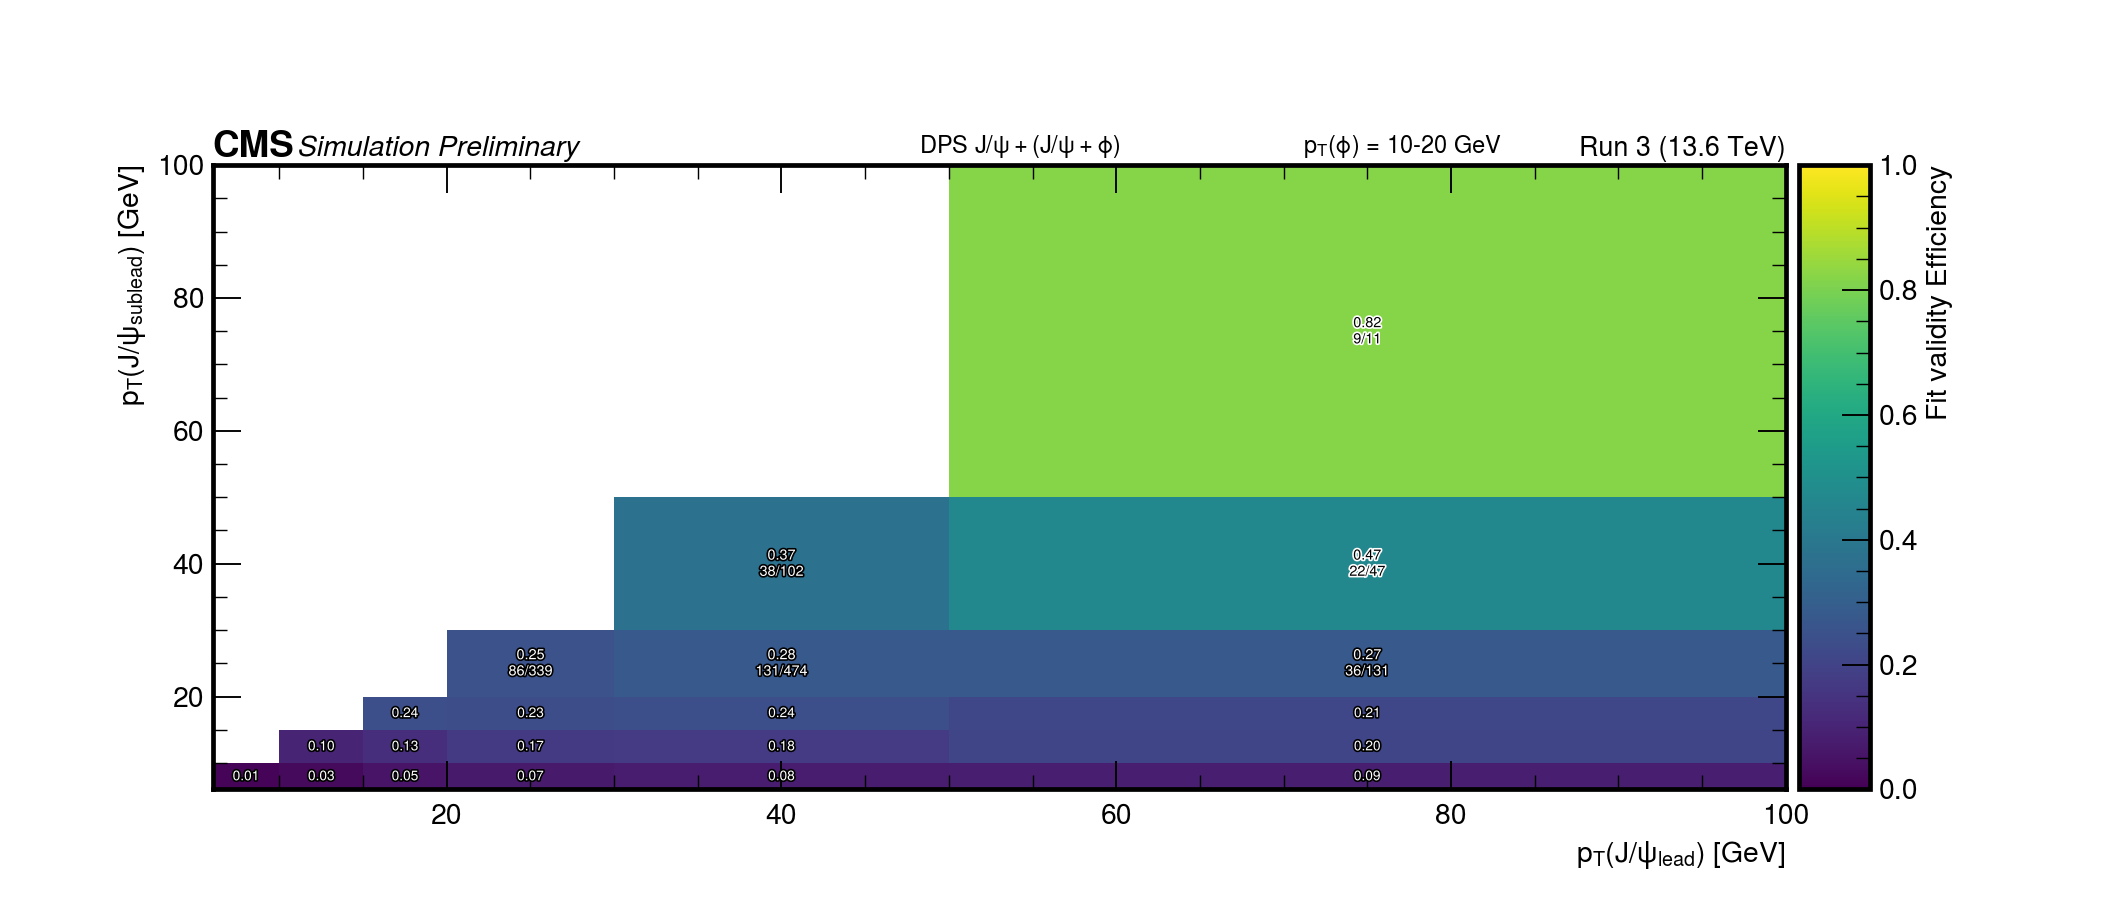
\includegraphics[width=0.85\textwidth]{figures/appendix-efficiency/corr3d_Pri_fitValid_phiPt_2.0.png}\\[2pt]
  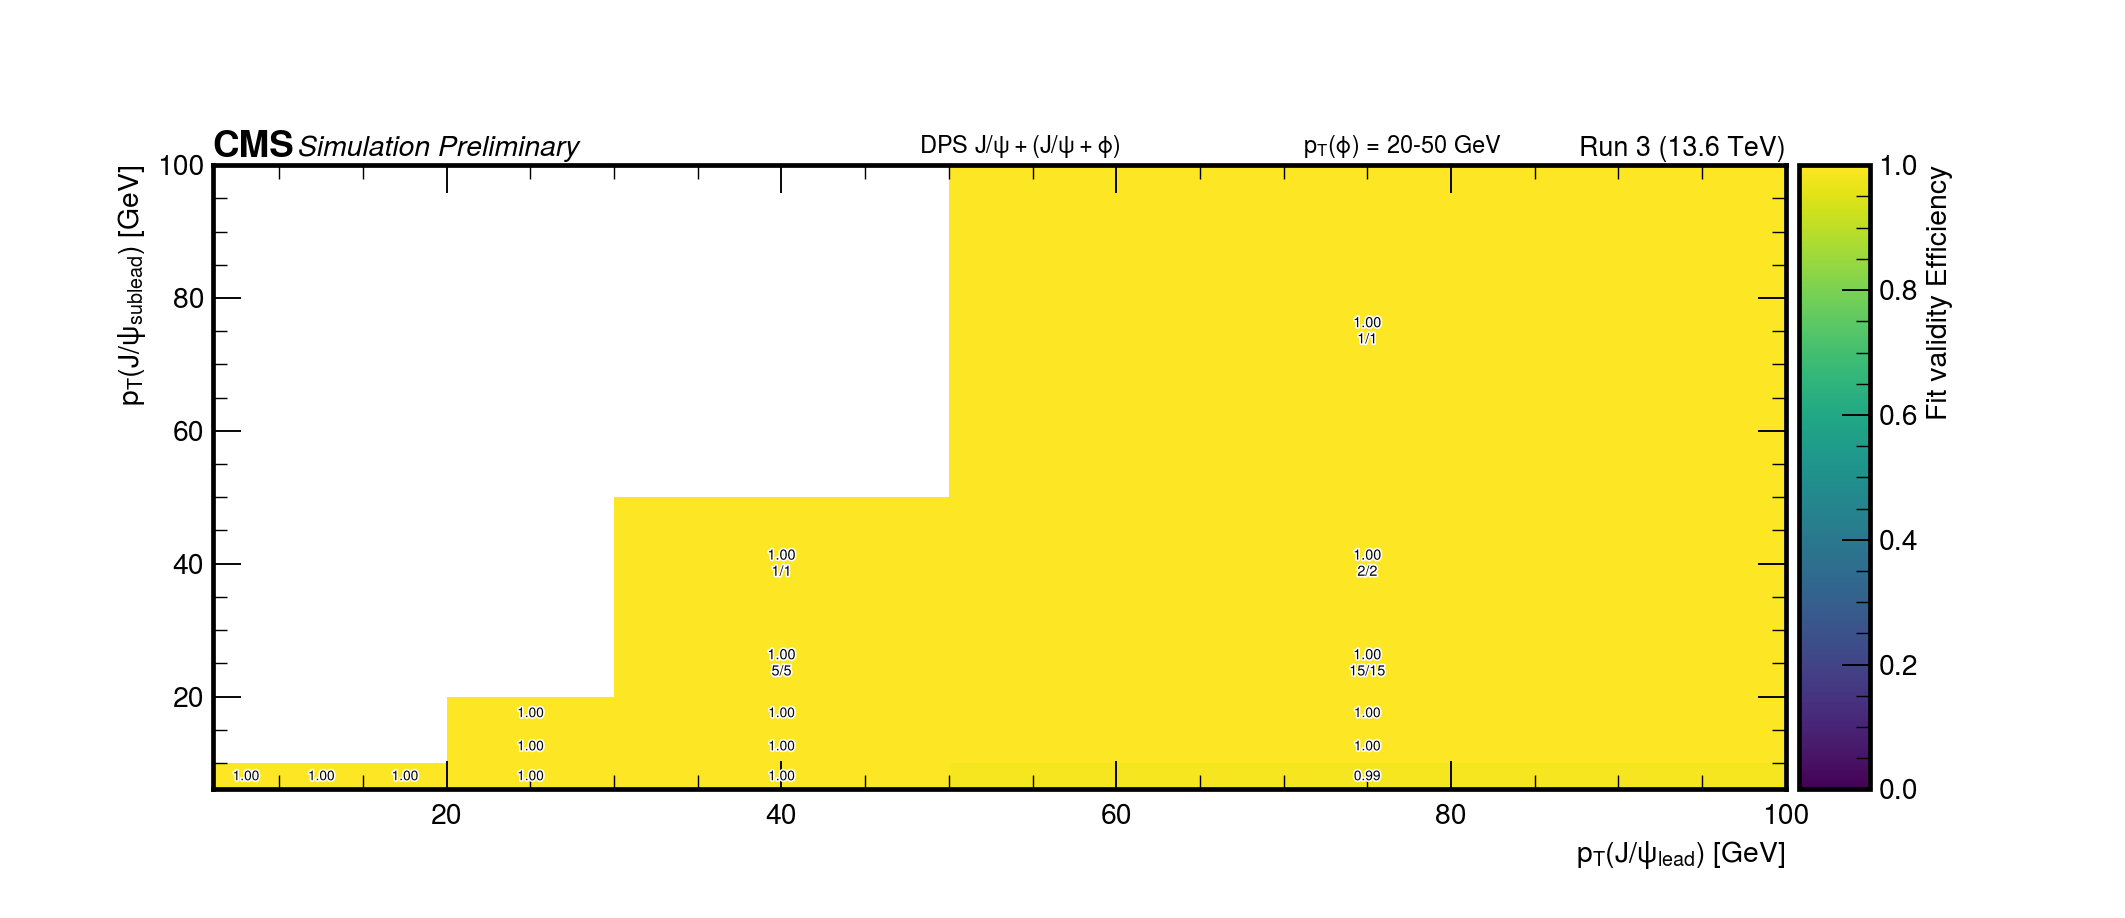
\includegraphics[width=0.85\textwidth]{figures/appendix-efficiency/corr3d_Pri_fitValid_phiPt_3.0.png}
  \caption{初级顶点有效性效率（$\epsilon_{\mathrm{Pri\_fitValid}}$）作为$p_{\mathrm{T}}(J/\psi_1)$和$p_{\mathrm{T}}(J/\psi_2)$的函数，按$p_{\mathrm{T}}(\phi)$区间分组。}
  \label{fig:app-eff-pri-fitvalid}
\end{figure}
